%% ----------------------------------------------------------------
%% Project.tex
%% ---------------------------------------------------------------- 
\documentclass{ecsproject}     
\usepackage[backend=bibtex8, style=ieee]{biblatex}
\usepackage{acro}
\usepackage[singlelinecheck=false]{caption}
\usepackage{booktabs}
\usepackage{float}
\usepackage{makecell}
\usepackage{subfig}
\usepackage{pgfgantt}
\usepackage{longtable}
\usepackage[shortlabels]{enumitem}
\usepackage{array}
\usepackage{multirow}
\usepackage{colortbl}
\usepackage[math]{cellspace}
\usepackage{amsmath}

\newcommand{\PreserveBackslash}[1]{\let\temp=\\#1\let\\=\temp}
\newcolumntype{C}[1]{>{\PreserveBackslash\centering}m{#1}}
\newcolumntype{R}[1]{>{\PreserveBackslash\raggedleft}m{#1}}
\newcolumntype{L}[1]{>{\PreserveBackslash\raggedright}m{#1}}
\newcommand{\centered}[1]{\begin{tabular}{l} #1 \end{tabular}}

%% ----------------------------------------------------------------
%% Definitions.tex
%% ---------------------------------------------------------------- 
\newcommand{\BibTeX}{{\rm B\kern-.05em{\sc i\kern-.025em b}\kern-.08em T\kern-.1667em\lower.7ex\hbox{E}\kern-.125emX}}

%% People
\newcounter{address}
\setcounter{address}{1}
\renewcommand{\theaddress}{\textsuperscript{\fnsymbol{address}}}
\newcommand{\address}[1]{\refstepcounter{address}\theaddress#1\\}
\newcommand{\Name}[3]{\texorpdfstring{\href{mailto:#3}{#2}#1}{#2}\xspace}
\newcommand{\DavidJones}[1]{\Name{#1}{David Jones}{dsj1n15@soton.ac.uk}}

%% Dingbats
\newcommand{\tick}{\ding{51}}
\newcommand{\cross}{\ding{55}}

%% Calculus
\newcommand{\pd}[2]{\ensuremath{\frac{\partial #1}{\partial #2}}\xspace}
\newcommand{\fd}[2]{\ensuremath{\frac{d #1}{d #2}}\xspace}
\newcommand{\dint}{\ensuremath{\int\!\!\!\int}\xspace}
\newcommand{\tint}{\ensuremath{\int\!\!\!\int\!\!\!\int}\xspace}

%% Math Sets
\newcommand{\Q}[1]{\ensuremath{\mathbb{#1}}\xspace}
\newcommand{\R}{\Q{R}}

%% Matrix, Vector
\newcommand{\V}[1]{\ensuremath{\boldsymbol{#1}}\xspace}
\newcommand{\M}[1]{\ensuremath{\boldsymbol{#1}}\xspace}
\newcommand{\0}{\V{0}}
\newcommand{\1}{\V{1}}
\newcommand{\I}{\M{I}}

%% Math Functions
\newcommand{\F}[1]{\ensuremath{\mathrm{#1}}\xspace}
\newcommand{\sgn}{\F{sgn}}
\newcommand{\tr}{\F{trace}}
\newcommand{\diag}{\F{diag}}

%% Math Names
\newcommand{\N}[1]{\ensuremath{\mathit{#1}}\xspace}

%% Data
\newcommand{\mc}[1]{\ensuremath{\mathcal{#1}}\xspace}
\newcommand{\Hyp}{\mc{H}}
\newcommand{\D}{\mc{D}}

%% Kernel
\newcommand{\K}{\M{K}}
\newcommand{\eins}{\texorpdfstring{\ensuremath{\epsilon}}{\textepsilon}-insensitive\xspace}
\newcommand{\e}{\ensuremath{\epsilon}\xspace}
\newcommand{\Bxi}{\ensuremath{\boldsymbol{\xi}}\xspace}
\newcommand{\Kanova}{\ensuremath{\mathit{K_{ANOVA}}}\xspace}
\newcommand{\Kspline}{\ensuremath{\mathit{K_{spline}}}\xspace}

%% Bayesian
\newcommand{\MP}{\ensuremath{\mathit{{\scriptscriptstyle \hspace{-1.5pt}M\hspace{-1.5pt}P}}}\xspace}
\newcommand{\ML}{\ensuremath{\mathit{{\scriptscriptstyle \hspace{-1.5pt}M\hspace{-1.5pt}L}}}\xspace}
\newcommand{\Qw}{\ensuremath{Q_{\w}(\w)}\xspace}
\newcommand{\Qa}{\ensuremath{Q_{\Ba}(\Ba)}\xspace}
\newcommand{\Qb}{\ensuremath{Q_{\beta}(\beta)}\xspace}
\newcommand{\wMPab}{\ensuremath{\w_{\MP|\bar {\Ba},\bar \beta}}\xspace}
\newcommand{\wMP}{\ensuremath{\w_{\MP}}\xspace}
\newcommand{\yMP}{\ensuremath{y_{\MP}}\xspace}
\newcommand{\BaMP}{\ensuremath{\Ba_{\hspace{1pt}\MP}}\xspace}
\newcommand{\aMP}{\ensuremath{\alpha_{\hspace{1pt}\MP}}\xspace}
\newcommand{\bMP}{\ensuremath{\beta_{\hspace{1pt}\MP}}\xspace}
\newcommand{\Sab}{\ensuremath{\M{\Sigma}_{\bar \Ba,\bar \beta}}\xspace}
\newcommand{\Ba}{\ensuremath{\boldsymbol{\alpha}}\xspace}
\newcommand{\Bb}{\ensuremath{\boldsymbol{\beta}}\xspace}
\newcommand{\Bm}{\ensuremath{\boldsymbol{\mu}}\xspace}
\newcommand{\BL}{\ensuremath{\boldsymbol{\Lambda}}\xspace}
\newcommand{\BPhi}{\ensuremath{\boldsymbol{\Phi}}\xspace}
\newcommand{\SMP}{\ensuremath{\M{\Sigma}_{\MP}}\xspace}

\newcommand{\Pa}{\ensuremath{P(\alpha|\mathcal{H})}\xspace}
\newcommand{\Pb}{\ensuremath{P(\beta|\mathcal{H})}\xspace}
\newcommand{\Pab}{\ensuremath{P(\alpha,\beta|\mathcal{H})}\xspace}
\newcommand{\Pw}{\ensuremath{P(\w|\mathcal{H})}\xspace}
\newcommand{\PD}{\ensuremath{P(\D|\mathcal{H})}\xspace}
\newcommand{\PwIa}{\ensuremath{P(\w|\alpha,\mathcal{H})}\xspace}
\newcommand{\PDIwb}{\ensuremath{P(\D|\w,\beta,\mathcal{H})}\xspace}
\newcommand{\PDwab}{\ensuremath{P(\D,\w,\alpha,\beta|\mathcal{H})}\xspace}
\newcommand{\PDIw}{\ensuremath{P(\D|\w,\mathcal{H})}\xspace}
\newcommand{\PwID}{\ensuremath{P(\w|\D,\mathcal{H})}\xspace}
\newcommand{\PwabID}{\ensuremath{P(\w,\alpha,\beta|\D,\mathcal{H})}\xspace}

\newcommand{\PanH}{\ensuremath{P(\alpha)}\xspace}
\newcommand{\PbnH}{\ensuremath{P(\beta)}\xspace}
\newcommand{\PabnH}{\ensuremath{P(\alpha,\beta)}\xspace}
\newcommand{\PwnH}{\ensuremath{P(\w)}\xspace}
\newcommand{\PDnH}{\ensuremath{P(\D)}\xspace}
\newcommand{\PwIanH}{\ensuremath{P(\w|\alpha)}\xspace}
\newcommand{\PDIwbnH}{\ensuremath{P(\D|\w,\beta)}\xspace}
\newcommand{\PDwabnH}{\ensuremath{P(\D,\w,\Ba,\beta)}\xspace}
\newcommand{\PDIwnH}{\ensuremath{P(\D|\w)}\xspace}
\newcommand{\PwIDnH}{\ensuremath{P(\w|\D)}\xspace}
\newcommand{\PwabIDnH}{\ensuremath{P(\w,\alpha,\beta|\D)}\xspace}

\newcommand{\PDwBab}{\ensuremath{P(\D,\w,\Ba,\beta|\mathcal{H})}\xspace}
\newcommand{\PwIBa}{\ensuremath{P(\w|\Ba,\mathcal{H})}\xspace}
\newcommand{\PBab}{\ensuremath{P(\Ba,\beta|\mathcal{H})}\xspace}
\newcommand{\PwBabID}{\ensuremath{P(\w,\Ba,\beta|\D,\mathcal{H})}\xspace}

\newcommand{\PBanH}{\ensuremath{P(\Ba)}\xspace}
\newcommand{\PwIBanH}{\ensuremath{P(\w|\Ba)}\xspace}

%% Snakes
\newcommand{\Esnake}{\ensuremath{\mathit{E_{snake}}}\xspace}
\newcommand{\Eimage}{\ensuremath{\mathit{E_{image}}}\xspace}
\newcommand{\Econt}{\ensuremath{\mathit{E_{cont}}}\xspace}
\newcommand{\Ecurv}{\ensuremath{\mathit{E_{curv}}}\xspace}
\newcommand{\Eint}{\ensuremath{\mathit{E_{int}}}\xspace}
\newcommand{\Eext}{\ensuremath{\mathit{E_{ext}}}\xspace}
\newcommand{\Eterm}{\ensuremath{\mathit{E_{term}}}\xspace}
\newcommand{\Eline}{\ensuremath{\mathit{E_{line}}}\xspace}
\newcommand{\Eedge}{\ensuremath{\mathit{E_{edge}}}\xspace}
\newcommand{\Econ}{\ensuremath{\mathit{E_{con}}}\xspace}
\newcommand{\Eangle}{\ensuremath{\mathit{E_{angle}}}\xspace}
\newcommand{\Elshape}{\ensuremath{\mathit{E_{lshape}}}\xspace}
\newcommand{\Eedgedir}{\ensuremath{\mathit{E_{edgedir}}}\xspace}
\newcommand{\Emodel}{\ensuremath{\mathit{E_{model}}}\xspace}
\newcommand{\wte}{\ensuremath{\mathit{w_{term}}}\xspace}
\newcommand{\wli}{\ensuremath{\mathit{w_{line}}}\xspace}
\newcommand{\wed}{\ensuremath{\mathit{w_{edge}}}\xspace}
\newcommand{\wco}{\ensuremath{\mathit{w_{con}}}\xspace}

%% Environments
\newcounter{alg}
\newenvironment{algorithm}[1]
{
    \stepcounter{alg}
    \begin{table}[htb]
    \centering
    \begin{tabular}[t]{ll}
    \hline&\\
    \multicolumn{2}{l}{\bf Algorithm \arabic{alg}: #1}\\&\\
} {
    &\\
    \hline
    \end{tabular}
    \end{table}
}

% class `abbrev': abbreviations:
\DeclareAcronym{lora}{
  short = LoRa,
  long  = \textbf{Lo}ng \textbf{Ra}nge (radio) ,
  class = abbrev
}

\DeclareAcronym{phy}{
  short = PHY,
  long  = \textbf{Phy}sical Layer,
  class = abbrev
}

\DeclareAcronym{csma}{
  short = CSMA,
  long  = \textbf{C}arrier-\textbf{s}ense \textbf{M}utliple \textbf{A}ccess,
  class = abbrev
}

\DeclareAcronym{macaw}{
  short = MACAW,
  long  = \textbf{M}ultiple \textbf{A}ccess with \textbf{C}ollision \textbf{A}voidance (for \textbf{W}ireless LANs),
  class = abbrev
}

\DeclareAcronym{pc}{
  short = PC,
  long  = \textbf{P}acket \textbf{C}ount,
  class = abbrev
}

\DeclareAcronym{eh}{
  short = EH,
  long  = \textbf{E}xplicit  \textbf{H}eader,
  class = abbrev
}

\DeclareAcronym{prp}{
  short = PRP,
  long  = \textbf{P}acket \textbf{R}eceive \textbf{P}ercentage,
  class = abbrev
}

\DeclareAcronym{mac}{
  short = MAC,
  long  = \textbf{M}edium \textbf{A}ccess \textbf{C}ontrol,
  class = abbrev
}

\DeclareAcronym{llbp}{
  short = LLBP,
  long  = \textbf{L}oRa \textbf{L}ocal \textbf{B}roadcast \textbf{P}rotocol,
  class = abbrev
}

\DeclareAcronym{td}{
  short = TD,
  long  = \textbf{T}est \textbf{D}efinition,
  class = abbrev
}

\DeclareAcronym{fspl}{
  short = FSPL,
  long  = \textbf{F}ree \textbf{S}pace \textbf{P}ath \textbf{L}oss,
  class = abbrev
}

\DeclareAcronym{pe}{
  short = PE,
  long  = \textbf{P}lain \textbf{E}arth,
  class = abbrev
}

\DeclareAcronym{sp}{
  short = SP,
  long  = \textbf{S}lave \textbf{P}osition,
  class = abbrev
}

\DeclareAcronym{mp}{
  short = MP,
  long  = \textbf{M}aster \textbf{P}osition,
  class = abbrev
}

\DeclareAcronym{ps}{
  short = PS,
  long  = \textbf{P}reamble \textbf{S}ymbols,
  class = abbrev
}

\DeclareAcronym{rps}{
  short = RPS,
  long  = \textbf{R}eceived \textbf{P}acket \textbf{S}trength,
  class = abbrev
}

\DeclareAcronym{los}{
  short = LOS,
  long  = \textbf{L}ine \textbf{o}f \textbf{S}ight,
  class = abbrev
}

\DeclareAcronym{olsr}{
  short = OLSR ,
  long  = \textbf{O}ptimised \textbf{L}ink \textbf{S}tate \textbf{R}outing (protocol),
  class = abbrev
}

\DeclareAcronym{lar}{
  short = LAR ,
  long  = \textbf{L}ocation \textbf{A}ided \textbf{R}outing (protocol),
  class = abbrev
}

\DeclareAcronym{aodv}{
  short = AODV ,
  long  = \textbf{A}d-Hoc \textbf{O}n \textbf{D}emand Distance \textbf{V}ector (protocol),
  class = abbrev
}

\DeclareAcronym{dtn}{
  short = DTN,
  long  = \textbf{D}elay \textbf{T}olerant \textbf{N}etwork ,
  class = abbrev
}

\DeclareAcronym{scf}{
  short = SCF,
  long  = \textbf{S}tore \textbf{C}arry \textbf{F}orward ,
  class = abbrev
}

\DeclareAcronym{rf}{
  short = RF,
  long  = \textbf{R}adio \textbf{F}requency,
  class = abbrev
}

\DeclareAcronym{crc}{
  short = CRC,
  long  = \textbf{C}yclic \textbf{R}edundancy \textbf{C}heck,
  class = abbrev
}

\DeclareAcronym{adr}{
  short = ADR,
  long  = \textbf{A}daptive \textbf{D}ata \textbf{R}ate,
  class = abbrev
}

\DeclareAcronym{psa}{
  short = PSA,
  long  = \textbf{P}olite \textbf{S}pectrum \textbf{A}ccess,
  class = abbrev
}

\DeclareAcronym{eirp}{
  short = EIRP,
  long  = \textbf{E}quivalent \textbf{I}sotropically \textbf{R}adiated \textbf{P}ower,
  class = abbrev
}

\DeclareAcronym{fcc}{
  short = FCC,
  long  = \textbf{F}ederal \textbf{C}ommunications \textbf{C}ommission,
  class = abbrev
}

\DeclareAcronym{dsss}{
  short = DSSS,
  long  = \textbf{D}irect \textbf{S}equence \textbf{S}pread \textbf{S}pectrum,
  class = abbrev
}

\DeclareAcronym{srd}{
  short = SRD,
  long  = \textbf{S}hort \textbf{R}ange \textbf{D}evice,
  class = abbrev
}


\DeclareAcronym{etsi}{
  short = ETSI,
  long  = \textbf{E}uropean \textbf{T}elecommunications \textbf{S}tandards \textbf{I}nstitute,
  class = abbrev
}


\DeclareAcronym{manet} {
  short = MANET ,
  long  = \textbf{M}obile \textbf{A}d-hoc \textbf{Net}work ,
  class = abbrev
}

\DeclareAcronym{lpwan}{
  short = LPWAN ,
  long  = \textbf{L}ow \textbf{P}ower \textbf{W}ide \textbf{A}rea \textbf{N}etwork,
  class = abbrev
}

\DeclareAcronym{lan}{
  short = LAN ,
  long  = \textbf{L}ocal \textbf{A}rea \textbf{N}etwork,
  class = abbrev
}

\DeclareAcronym{wan}{
  short = WAN ,
  long  = \textbf{W}ide \textbf{A}rea \textbf{N}etwork,
  class = abbrev
}

\DeclareAcronym{lte}{
  short = LTE ,
  long  = \textbf{L}ong-\textbf{T}erm \textbf{E}volution,
  class = abbrev
}

\DeclareAcronym{css}{
  short = CSS ,
  long  = \textbf{C}hirp \textbf{S}pread \textbf{S}pectrum,
  class = abbrev
}

\DeclareAcronym{sf}{
  short = SF ,
  long  = \textbf{S}preading \textbf{F}actor,
  class = abbrev
}

\DeclareAcronym{bw}{
  short = BW ,
  long  = \textbf{B}and\textbf{w}idth,
  class = abbrev
}

\DeclareAcronym{cr}{
  short = CR ,
  long  = \textbf{C}oding \textbf{R}ate,
  class = abbrev
}
\DeclareAcronym{ism}{
  short = ISM ,
  long  = {\textbf{I}ndustrial, \textbf{S}cience, Medical} ,
  class = abbrev
}

\DeclareAcronym{fec}{
  short = FEC ,
  long  = {\textbf{F}orward \textbf{E}rror \textbf{C}orrection} ,
  class = abbrev
}

\DeclareAcronym{cad}{
  short = CAD,
  long  = {\textbf{C}hannel \textbf{A}ctivity \textbf{D}etection} ,
  class = abbrev
}

\DeclareAcronym{rssi}{
  short = RSSI ,
  long  = \textbf{C}oding \textbf{R}ate,
  class = abbrev
}
\DeclareAcronym{snr}{
  short = SNR ,
  long  = {\textbf{S}ignal-\textbf{N}oise-\textbf{R}atio} ,
  class = abbrev
}

\DeclareAcronym{per}{
  short = PER ,
  long  = {\textbf{P}acket \textbf{E}rror \textbf{R}ate} ,
  class = abbrev
}

\DeclareAcronym{ber}{
  short = BER ,
  long  = {\textbf{B}it \textbf{E}rror \textbf{R}ate} ,
  class = abbrev
}

\DeclareAcronym{cf}{
  short = CF ,
  long  = {\textbf{C}arrier \textbf{F}requency} ,
  class = abbrev
}

\DeclareAcronym{pl}{
  short = PL ,
  long  = {\textbf{P}acket \textbf{L}ength} ,
  class = abbrev
}

\DeclareAcronym{tp}{
  short = TP ,
  long  = {\textbf{T}ransmit \textbf{P}ower} ,
  class = abbrev
}

\DeclareAcronym{lorawan}{
  short = LoRaWAN ,
  long  = {\textbf{Lo}ng \textbf{Ra}nge \textbf{W}ide \textbf{A}rea \textbf{N}etwork} ,
  class = abbrev
}

\DeclareAcronym{rtc}{
  short = RTC ,
  long  = {\textbf{R}eal \textbf{T}ime \textbf{C}lock} ,
  class = abbrev
}
\DeclareAcronym{lipo}{
  short = Li-Po,
  long  = \textbf{Li}thium \textbf{Po}lymer (battery),
  class = abbrev
}

\graphicspath{{../Figures/}}
\hypersetup{colorlinks=false}
\acsetup{first-style=short}
\bibliography{citations}

%% ----------------------------------------------------------------
\begin{document}
\frontmatter
\title      {LoRa Communications for Sparse Robot Swarms}
\authors    {\texorpdfstring
             {\href{mailto:dsj1n15@soton.ac.uk}{David Jones}}
             {David Jones}
            }
\addresses  {\groupname\\\deptname\\\univname}
\date       {\today}
\subject    {}
\keywords   {}
\supervisor {Dr Klaus-Peter Zauner}
\examiner   {Prof. Kirk Martinez}
\degree     {MEng Computer Science}
\maketitle

\begin{abstract}


\end{abstract}

\tableofcontents
\listoffigures
\listoftables
%\lstlistoflistings


\chapter{Acronyms}
\vspace{-20mm}
\printacronyms[include-classes=abbrev, name=]
\printacronyms[include-classes=radio_params, name=]

\input{Symbols}
\acknowledgements{
This work would not have been possible without Klaus Peter-Zauner's weekly guidance and continuous support. I am also thankful to Kirk Martinez for his invaluable suggestions on simulation methods, which kept this project progressing. Most of all I would like to thank any family and friends who kept me company through the many hours of data collection, no matter the weather!
}
\mainmatter

%% ----------------------------------------------------------------
\chapter{Introduction}
Decentralisation of wireless control and data sharing systems allows flexible deployment structures over large areas. Conversely, using a single centralised node, deployments are limited by that node's placement and its maximum communication range. This paper studies the application of \ac{lora}, an emerging long range, low power, radio frequency (\ac{rf}) technology, for the decentralised use case of sparse robot swarms. Solutions are targeted at and scenarios are devised from the use case, however as the research topics discussed are applicable to many areas, descriptions are largely kept agnostic. 
  
Swarm robotics is the coordination of multi-robot systems such that a common goal can be achieved. Capabilities of a swarm should exceed that of any single robot in the swarm; be that attributed to increased coverage \cite{Ducatelle:2011:Pathfinding} or self-assembly methods \cite{3YP:OBSTACLE_SWARMS}. 
%Robots will often have differing hardware/payloads so that either multiple terrain types can be handled, or to reduce robot costs (one robot need not possess all sensor types).
 Although spreading robots across large areas opens up potential for many practical applications, including terrain mapping, and search and rescue, the sophistication of robots required in these real-world scenarios can make them prohibitively expensive, which can lead to limited robot density. These are referred to as sparse swarms. For the sake of perspective this paper assumes distances that are beyond the capabilities of typical short-range communications such as Wi-Fi.
 
Unlike a centralised control approach, swarms rely on robots sharing data directly so that all instances can build a combined interpretation of the environment. Although some data may need to be decimated to many or all robots in the network, the vast majority will only be of interest to physically local neighbours. Global interest data may be for swarm management, e.g. voting decisions, or be generic, e.g. battery usage figures for specific terrain fingerprints. Whereas, local interest data may be found obstacles or robot routes. In critical scenarios, for example when robot failure is impending, large fast data dumps may be required. Alternatively, data can be continuously aggregated and distributed in a BitTorrent-like fashion \cite{3YP:SOUL}.

For concentrated deployments, these scenarios are trivial to implement using high-data-rate technologies such as Wi-Fi. However, in a real-world scenario, when inter-robot distance is significant, and there are line of sight (\ac{los}) obstructions (e.g. trees), an alternative physical medium is required. This leads to the choice of \ac{lora}, detailed in Section \ref{sec:lora}. The system can be considered as a mobile-ad-hoc-network (\ac{manet}), due to the ever changing topology caused by internal system changes (e.g. robot movement), or external system changes (e.g. weather).

Although \ac{lora} is fundamentally ideal for long-range applications and operates in the low attenuation Sub-1GHz band, scenario specific conditions of ground-level transmissions and high-propagation environments are not ideal for \ac{rf} communications. Therefore this project initially covers real-world testing in free-space and forests to assess how sparse swarm deployment scenarios may affect \ac{lora}'s physical radio performance. From this, demodulation models are extracted and combined with \ac{lora} collision models from literature to create a simulator for testing \ac{lora} ad-hoc scenarios. This simulator is used to analyse the effectiveness of three \ac{mac} protocols with the aim of prioritising data distribution to physically local neighbours. Two methods utilise common approaches (ALOHA and \ac{csma}), and the third attempts to exploit hardware parameters and regional \ac{rf} regulations; this is defined as the LoRa Local Broadcast Protocol (\ac{llbp}).

%Alongside the physical communication medium, a  is needed.
%Many MAC layer protocols exist 
%\cite{3YP:FLOCK_1, 3YP:FLOCK_2, 3YP:FLOCK_3}
%Separation distance is less of an issue as much existing work covers guaranteeing minimum connectivity via positioning !!!.

%Power usage must be proportionate to that of the overall robot,  i.e. power usage can exceed that of nodes in a fixed-position sensor network but not extend to long range Wi-Fi. In a real-world scenario the communications must be robust to physical environmental changes, which can stem from circumstances that are either external to the system, such as weather, or internal to the system, such as robot positioning. The latter having resulting factors such as varying separation distance or change in line of sight propagation caused by obstacles (e.g. trees and ridges). Wi-Fi signals in the 2.4GHz or 5GHz bands are easily attenuated so an alternative physical medium is required; this leads to the choice of \ac{lora}, which operates in the Sub-1GHz band.

%If radio hardware is designed for a worst case scenario, the throughput for normal situations will ve greatly impaired. If the hardware is designed for an average situation. the network risks partition under stress because of poor radio links.

%The target should be to minimise airtime. Longer airtime increases collision chance and reduces throughput of the network as a whole.
\chapter{Background}
\section{\ac{lora}}
\subsection{Overview}
LoRa is a physical long-range, low-power, communication technology developed and patented by Semtech\footnote{Semtech, USA, https://www.semtech.com/}. It is designed to operate inside varying unlicensed \ac{ism} bands worldwide. Consequently, under the proviso that local regulatory standards are obeyed (see Section \ref{sec:ISMBandRegulation}), it can be used for wide area deployments without being tied to expensive licensed carriers. Fundamentally, even using its fastest configuration, it is a low-data rate modulation technique. Performance calculations provided are based on Semtech's current LoRa transceiver designs (SX1276/77/78/79) \cite{3YP:LORA_SX12}.

Long-range communication can be a challenge in the \ac{ism} bands as the heavy congestion can result in a high physical noise floor. This being the sum of all signals in the band from sources such as the atmosphere or radio devices, excluding that of the signal being monitored. \ac{lora} is one solution to this, it functions using a unique chirp spread spectrum (\ac{css}) modulation technique that can operate below the noise floor. Spread spectrum techniques allow signal-to-noise degradation in a single channel to be compensated for by spreading across other channels. Unlike other \ac{css} techniques that use a fixed chip sequence to carry out spreading, \ac{lora} modulation uses a chirp signal that varies in frequency continuously; this allows the complexity of the receiver design to be greatly reduced and has resulted in a reduced and accessible hardware cost \cite{3YP:LORA_MOD_BASICS}.

The modulation technique means \ac{lora} can boast a far more adaptive and efficient link budget compared to frequency shift keying (FSK) and other modulation types \cite{3YP:LORA_MOD_BASICS}. The link budget being the measure of all gains and losses incurred by a signal passing through the transmitter, the receiver and the propagation channel. This equation in its simplest form is as follows:
\begin{equation}
\label{link_budget}
RX\ Power\ (dB)\ = TX\ Power\ (dB)\ +\ Gains\ (dB)\ -\ Losses\ (dB)
\end{equation}

\subsection{Parameters}
\ac{lora} hardware has many parameters that can be configured to extend range or increase reliability at the expense of air time, data-rate or energy consumption. These are independent from any external hardware and include:
\begin{itemize}
    \item \textbf{Bandwidth (\ac{bw})}: The range of the chirps around the \ac{cf}. Increasing bandwidth increases data-rate but decreases receiver sensitivity \cite{3YP:STUDY_OF_LORA}.
    \item \textbf{Carrier frequency (\ac{cf})}: The centre frequency of chirps. Current hardware targets some sub-range of 137MHz to 1020MHz at a resolution of 61Hz \cite{3YP:LORA_SX12}. 
    \item \textbf{Coding rate (\ac{cr})}: The amount of redundant information encoded in symbols for forward error correction (\ac{fec}); trade-offs can be seen in Table \ref{cr_effect}.
    \item \textbf{Preamble length (\ac{pl})}: The header length of a sent packet used to synchronise transmission. Packet error rate (\ac{per}) has been shown to decrease with an increased \ac{pl} up to a certain threshold \cite{3YP:LORA_PERFORMANCE}. Increasing length can also improve performance of \ac{cad} (see Section \ref{sec:cad}).
    \item \textbf{Spreading factor (\ac{sf})}: The ratio of chip rate to bit rate, where chips per symbol is given as $2^{SF}$. Receiver sensitivity increases in line with spreading factor and is therefore a factor in the link budget \cite{3YP:LORA_SX12}. The trade-offs can be seen in Table \ref{sf_effect}.
    \item \textbf{Transmission power (\ac{tp})}: The radio output power. Equation \ref{link_budget} highlights how an increased \ac{tp} directly increases link budget with the obvious drawback of higher power usage.
\end{itemize}
Figure \ref{lora_transmission_structure} highlights how these parameters affect the structure of a \ac{lora} transmission. The effect on airtime is explained in Section \ref{sec:LoRaTiming}.

\begin{table}
\centering\small
\caption[Effect of \ac{cr}s on \ac{lora} transmissions]{Effect of \ac{cr}s on \ac{lora} transmissions. Recovery performance is defined as the best case percentage of bits that can be lost for a successful receive. \\ Compiled from data in \cite{3YP:LORA_PERFORMANCE}.}
\label{cr_effect}
\begin{tabular}{c|cc}
    \toprule
    \textbf{Coding Rate} & \textbf{Data Overhead} & \textbf{Recovery}  \\
    \midrule\addlinespace
    4/5 & $\times$1.25 & 20\% \\
    4/6 & $\times$1.50 & 33\% \\
    4/7 & $\times$1.75 & 43\% \\
    4/8 & $\times$2.00 & 50\% \\
    \addlinespace\bottomrule
\end{tabular}
\end{table}

\begin{table}
\centering\small
\caption[Effect of \ac{sf} on \ac{lora} transmissions]{Effect of \ac{sf} on \ac{lora} transmissions (\ac{bw}=125KHz). Compiled from data in \cite{3YP:LORA_MOD_BASICS} and \cite{3YP:LORA_PERFORMANCE}.}
\begin{tabular}{c|ccc}
    \toprule
    \makecell{\textbf{\ac{sf}} \\ \textbf{(\ac{lora} Mode)}} & \makecell{\textbf{\ac{sf}} \\ \textbf{(Chirps / Symbol)}} & \makecell{\textbf{Bit Rate} \\ \textbf{(bits / sec)}} & \makecell{\textbf{Demodulation Limit} \\ \textbf{(\ac{snr} dBm)}} \\
    \midrule\addlinespace
    SF7 & 128 & 5469 & -7.5 \\
    SF8 & 256 & 3125 & -10.0 \\
    SF9 & 512 & 1758 & -12.5 \\
    SF10 & 1024 & 977 & -15.0 \\
    SF11 & 2048 & 537 & -17.5 \\
    SF12 & 4096 & 293 & -20.0 \\
    \addlinespace\bottomrule
\end{tabular}
\label{sf_effect}
\end{table}
Selection of these parameters will often be manual, however mechanisms such as \ac{adr} (see Section \ref{sec:lorawanADR}) or ``probing algorithms'', as proposed by \cite{3YP:CHOOSING_LORA_PARAMETERS}, can be used to choose these parameters such that transmission energy is reduced whilst maintaining an adequate throughput and link budget. These methods, due to their overhead, are most suited to static nodes communicating with a gateway.

\begin{figure}[H]
    \centering
   	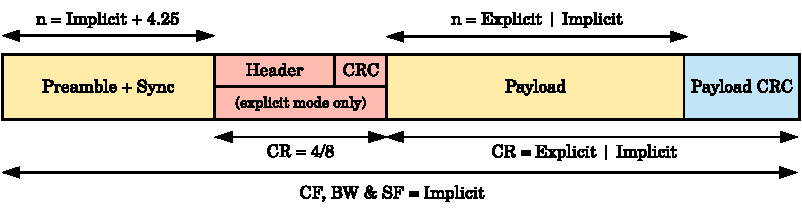
\includegraphics{Figures/lora_transmission.pdf}
    \caption[\ac{lora} transmission packet structure]{
    Structure of a standard \ac{lora} transmission. All transmissions contain a preamble, sync words, and a payload. The header section (in red) is optional but if present, contains information such as the payload length, the payload coding rate, and whether the \ac{crc} is present. If the header is not present this information must be fixed implicitly by the receiver. Parameters that are not in the header are always implicit and must match between transmitter and receiver (i.e. \ac{pl}, \ac{sf}, \ac{bw} and \ac{cf}). Adapted from \cite{3YP:LORA_SX12}.
    }
    \label{lora_transmission_structure}
\end{figure}

\subsection{Considerations}
It should be noted that \ac{lora} radios, like all current consumer radios, are half-duplex, meaning that they are unable to receive during transmission; this can result in missed receives. Consideration should also be given for the differing technology in transceivers and gateways. A gateway contains a \ac{lora} concentrator block, allowing demodulation of up to eight signals concurrently provided they use unique spreading factors \cite{3YP:LORA_SX1301}. A transceiver can only demodulate one signal at a time \cite{3YP:LORA_SX12}. Collisions may occur in the presence of conflicting signals, resulting in failed receives; the conditions of this occurrence are assessed further in Section \ref{sec:RadioCollisions}. Most \ac{lora} applications consist of many sensor nodes infrequently sending data to a single gateway with very little downlink; this means collisions and missed receives are rare. Unfortunately, in a mesh-like point-to-point network, these events are a very real possibility. High data-rate wireless communications, such as Wi-Fi, will often use carrier-sense multiple access (CSMA) mechanisms to allow for full-duplex emulation, but with LoRa this can lead to a waste of precious available airtime. Nonetheless, implementations using LoRa's \ac{cad} have been attempted with promising results for a single point-to-point transmission \cite{3YP:LORA_CSMA}. Though gateways are clearly more powerful than transceivers, their cost and power usage make them hard to deploy on scale. That being said, Pycom's\footnote{Pycom, UK,  https://pycom.io/} newly released Pygate gateway is a fraction of the cost of existing implementations and may be feasible for an ad-hoc scenario.
\subsection{Channel Activity Detection (\ac{cad})}\label{sec:cad}
Carrier-sensing is a helpful mechanism for radios to check whether a channel is busy or idle. Usually, this is achieved by checking the power present in the channel using the received signal strength indicator (\ac{rssi}). This is a very unreliable method for \ac{lora} because the \ac{rssi} includes channel noise, and \ac{lora} signals can operate below the noise floor. For this reason, \ac{lora} radios offer a specialised \ac{cad} method, which searches the channel for a single \ac{lora} packet preamble symbol. \ac{cad} is at least 97\% reliable in the presence of preamble with false positives occuring just 0.1\% of the time \cite{3YP:LORA_FOR_IOT}. It has been shown that \ac{cad} can in fact detect non-preamble symbols when there is high signal strength, although this ability quickly becomes unreliable in a real world scenario \cite{Pham:2018:CSMA}.

\subsection{Signal Orthogonality}
The manner of \ac{lora}'s modulation allows multiple signals to co-exist in the same channel provided they have a different chirp rate ($C_R$), where $C_R = BW \times S_R$. $S_R$ (symbol rate) is calculated as the chip rate, which is directly defined by the \ac{bw}, divided by the number of chips per symbol, $S_R=\frac{BW}{2^{SF}}$. This clearly demonstrates that for a single bandwidth, all \ac{sf}s must be orthogonal to one another. However, in the case that different \ac{bw}s are used, different \ac{sf}s may have the same chirp rate and could interfere; this is demonstrated in Figure \ref{fig:orthogonality}.

\begin{figure}[H]
    \centering
   	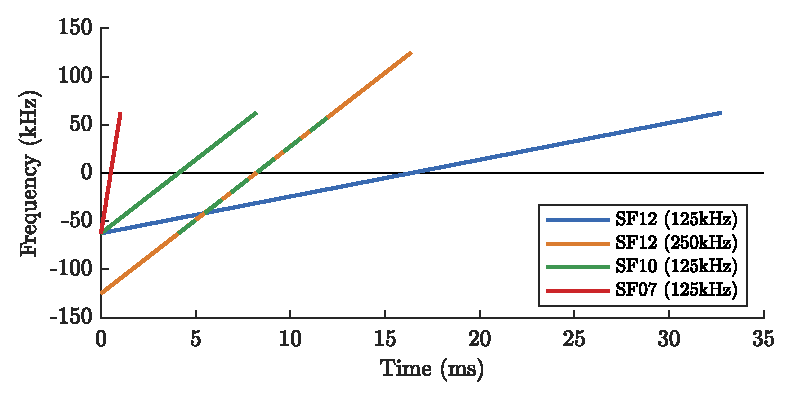
\includegraphics{Figures/sf_orthogonality_plot.eps}
    \caption[Signal chirp rate orthogonality]{
    Demonstration of signal orthogonality for different \ac{sf}s. The SF10 (125kHz) chirp is duplicated and shifted to overlap with the  SF12 (250kHz) chirp to highlight that they have the same chirp rate and are therefore not orthogonal.
    }
    \label{fig:orthogonality}
\end{figure}
%Symbol duration is the inverse of the symbol rate, defined in \ref{cr_effect}


\section{\ac{lorawan}}\label{sec:lorawanADR}
\ac{lorawan} is a MAC layer protocol designed to be the de facto choice for point-to-multipoint \ac{lora} applications. It is largely certified worldwide, open-source, and is both managed and promoted by the LoRa Alliance\footnote{Lora Alliance,  https://lora-alliance.org/}. The expectation of a star topology means the full protocol is not suited to the sparse swarm scenario, however, individual features are of interest. In principle it is implemented as Pure ALOHA (P-ALOHA) - a simple unchecked protocol where transmission occurs whenever a transmitter has data available to send. Figure \ref{fig:lorawan_duty_cycles} explains how duty cycle limits are enforced. The unchecked approach reduces theoretical channel usage to just 18\% \cite{3YP:LORAWAN_SLOTTED}. \ac{lorawan} abstracts \ac{sf}s and \ac{bw}s into a set of orthogonal data-rates where lower data-rates have higher range \cite{3YP:LORAWAN_REGIONAL_PARAMS}.

\begin{figure}[H]
    \centering
   	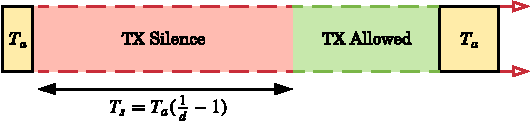
\includegraphics{Figures/duty_cycle_lorawan.pdf}
    \caption[\ac{lorawan} duty cycle enforcement]{
    Demonstration of how \ac{lorawan} enforces duty cycle limits; that is after a transmission of airtime $T_a$, the transmitter must be silent for a minimum period of $T_s=T_a(\frac{1}{d}-1)$ \cite{3YP:LIMITS_OF_LORAWAN}. The figure is to scale for $d=10\%$.
    
    }
    \label{fig:lorawan_duty_cycles}
\end{figure}


Optionally, \ac{tp}, \ac{sf} and \ac{bw} can be managed dynamically using \ac{lorawan}'s adaptive data-rate (ADR) functionality. Full technical detail is available in \cite{3YP:LORAWAN}, a brief overview follows. Operation is scheduled by a node setting the reserved \ac{adr} bit in uplink messages. The gateway responds with initial transmission parameters to attempt. The node sets its transmission parameters to these values and proceeds with the expectation that the gateway is reachable. However, if the gateway does not acknowledge any packets within a set period, the \ac{adr} bit is set again to force an acknowledgement. Failure to receive any acknowledgement implies that the gateway is not within range. Data-rate is reduced or \ac{tp} is increased until an acknowledgement is made, these are the parameters used unless a further \ac{adr} request is made. It has been suggested that the system has low-scalability due to packet count requirements \cite{3YP:LORAWAN_ADR} and is slow to converge \cite{3YP:LORAWAN_ADR_AGILITY}. Like \cite{3YP:CHOOSING_LORA_PARAMETERS}, this makes it only suitable for static nodes in a gateway controlled network.
\section{\ac{ism} Band Regulation}\label{sec:ISMBandRegulation}
The industrial, scientific and medical (\ac{ism}) bands are portions of the radio spectrum, which can be used without a license, subject to local regulatory standards. These standards vary around the world but often define maximum power outputs, duty cycles, and bandwidths. Though limits can be problematic, they help reduce the chance of internal and external system interference. Some of the most stringent regulations are in Europe, where they are controlled firstly by the European Telecommunications Standards Institute (the \ac{etsi}\footnote{ETSI, EU, https://www.etsi.org}), and then by country specific authorities. The United States' regulations are managed by the Federal Communications Commission (the \ac{fcc}\footnote{FCC, US, https://www.fcc.gov}), with many other countries following their example. 

Sub-1GHz \ac{lora} hardware operates around the 433MHz and 900MHz bands, but as the former is very heavily regulated for non-remote controls in the US \cite{3YP:FCC_433}, only the 900MHz area is considered viable to the use case. It should be noted however that the specific frequencies used will still differ between region, as is demonstrated by \ac{lorawan}'s use of the 863-870 MHz and 902-928 MHz bands for Europe and the US respectively \cite{3YP:LORAWAN_REGIONAL_PARAMS}. A comparison of the regulations can be seen in Table \ref{tab:ISMRegions}. As \ac{etsi} limits vary heavily on a by band basis, they are broken down further in Table \ref{tab:ETSIBands}. An overview of each regulation type follows.
 
\begin{table}[H]
\centering\small
\caption[900MHz regional regulation comparison]{Regional regulation comparison for 900MHz band radio \cite{3YP:FCC_900, 3YP:ETSI_HARMONISED_REG}.}
\label{tab:ISMRegions}
\renewcommand*{\arraystretch}{1.1}
\begin{tabular}{l|L{45mm}L{45mm}}
    \toprule
    & \textbf{\ac{fcc}} & \textbf{\ac{etsi}}  \\
    \midrule\addlinespace
    \textbf{Band} & 902--928MHz & 863--870MHz \\
    \textbf{\ac{eirp}} & {36dBm \newline \textit{  30dBm transmit power}} & {0.25MHz @ 27dBm \newline 6.40MHz @ $\leq$ 14dBm} \\
    \textbf{Duty Cycle} & None & 0.1\%--10\% \\
    \textbf{Bandwidth} & 26 MHz & 6.65MHz \\
    \textbf{Narrowband} & 400ms airtime per transmit & None\\
    \textbf{\ac{css}} & None & Varies  \\
    \addlinespace\bottomrule
\end{tabular}
\end{table}

Duty cycle limits greatly reduce the amount of airtime a radio is allowed. For example, in Band h1.3, there is a 1\% duty cycle, which indicates a maximum of 36 seconds of airtime, over all the band's channels, over a rolling one hour period. Duty cycles are considered within a band so a multi-band implementation may obey multiple duty cycles separately. Alternatively, the polite spectrum access (\ac{psa}) policy can be used; this is a defined regulation for listen before talk (LBT) implementations \ac{psa} allows airtime of up to 100 seconds per 200kHz of spectrum, per hour, regardless of duty cycle \cite{3YP:ETSI_PSA}. It does however require a clear channel assessment to be carried out before every transmission, this would be independent of \ac{lora}'s \ac{cad}.
 
\begin{table}
\centering\small
\caption[\ac{etsi} 868MHz sub-band breakdown]{\ac{etsi} 868MHz sub-bands for short range devices (adapted from \cite{3YP:ETSI_HARMONISED_REG}). Only bands relevant for \ac{css} are included. Band numbers correspond to CEPT-ERC-REC 70-03 definitions \cite{3YP:CEPT_ERC_REC}}
\label{tab:ETSIBands}
\renewcommand*{\arraystretch}{1.1}
\begin{tabular}{c|ccccc}
    \toprule
    \textbf{Band} & \textbf{Frequency} (MHz) & \textbf{\ac{eirp}} (dBm)  & \textbf{Duty Cycle} & \textbf{Max \ac{bw}} (kHz) \\
    \midrule\addlinespace
    \textbf{h1.2} & 863.00--870.00 & 14 & 0.1\% (or PSA) & 7000 \\
    \textbf{h1.3} & 865.00--868.00 & 14 & 1\% (or PSA) & 300 \\
    \textbf{h1.4} & 868.00--868.60 & 14 & 1\% (or PSA) & 600 \\
    \textbf{h1.5} & 868.70--869.20 & 14 & 0.1\% (or PSA) & 500 \\
    \textbf{h1.6} & 869.40--869.65 & 27 & 10\% (or PSA) & 250 \\
    \textbf{h1.7a} & 869.70--870.00 & 7 & None & 300 \\
    \textbf{h1.7b} & 869.70--870.00 & 14 & 1\% (or PSA) & 300 \\   
    \addlinespace\bottomrule
\end{tabular}
\end{table}

Regulations consider power as equivalent isotropically radiated power (\ac{eirp}). This value is directly related to radio transmission power ($P_t$) and can be calculated as $EIRP = P_t - L + G$ where $L$ is cable loss and $G$ is antenna gain. The latter occurring from transmit power being concentrated into a smaller area, all antenna will have some form of gain as isotropic antennas are only hypothetical. For example, a radio operating in Band h1.3, using a typical omnidirectional antenna that has 3dBi of gain, can only transmit at 11dBm if no cable loss occurs. Realistically, some cable loss will occur but this must be considered on an implementation by implementation basis. Directional antenna compound these issues due to their high-gains and the relatively low \ac{eirp} limits.

The \ac{etsi} regulations are the limiting factor in transmit power, duty cycle and overall available bandwidth. \ac{lora} being a \ac{css} signal means \ac{fcc} narrowband limitations need not be a concern. Under this consideration, the \ac{etsi} regulations will be used as the worst-fit scenario from here on in. When considering national regulation, it is common that either all bands are implemented, or none at all \cite{3YP:CEPT_ERC_REC}. Of the ETSI bands, h1.3, h1.4 and h1.6 are of most interest. h1.3 and h1.4 giving a balanced offering of bandwidth, \ac{eirp} and duty cycle. Whilst h1.6 offers a far greater duty cycle and \ac{eirp} but limited bandwidth; a further regulatory limit means only allows a single wide-band channel can operate within this band. The maximum number of possible \ac{lora} channels in each of these bands can be seen in Table \ref{tab:ETSILoraChannels}.

\begin{table}[H]
\centering\small
\caption[Maximum channel breakdown for \ac{lora}]{Maximum channel count breakdown for relevant \ac{etsi} bands, calculated for \ac{lora}'s most common operating bandwidths. Calculated assuming channel spacing is 120\%  of the bandwidth to avoid inter-channel interference.}
\label{tab:ETSILoraChannels}
\renewcommand*{\arraystretch}{1.1}
\begin{tabular}{c|ccc}
    \toprule
    & \multicolumn{3}{c}{\textbf{Channel \ac{bw}}}	\\
    \textbf{Band} & \textbf{125kHz} & \textbf{250kHz} & \textbf{500kHz}\\
    \midrule\addlinespace
    \textbf{h1.3} & 19 & 8 & N/A \\
    \textbf{h1.4} & 4 & 2 & 1 \\
    \textbf{h1.6} & 1 & 1 & 0 \\
    \addlinespace\bottomrule
\end{tabular}
\end{table}

\section{Ad-Hoc Networks}\label{sec:adhocnetworks}
\subsection{Routing}
An ad-hoc network is a type of wireless network that does not rely on managed infrastructure. The network's nodes are responsible for determining their own routing paths and forwarding other nodes packets (i.e. acting as the routers).  A \ac{manet}, is a type of ad-hoc network where nodes are expected to move, resulting in frequent changes to the network topology \cite{3YP:MANET_RFC2501}. If a network is sparse or operating at the limits of the transmission medium, and packet delivery is not time critical, the network can be treated as a delay-tolerant-network (\ac{dtn}). A common approach is to adopt store-carry-forward (\ac{scf}) behaviour; this is where intermediate nodes will keep hold of data until either a new path appears or signal strength improves \cite{3YP:DTNS}. A major requirement of ad-hoc networks, and the most researched  topic, is route management \cite{3YP:MANET_RESEARCH_TRENDS}. However, as this paper focuses on local broadcasts, the topic is not considered further, instead the reader is directed towards \cite{3YP:ROUTING_ALGORITHMS}.  

\subsection{\ac{mac} Protocols}
\label{sec:mac_protocol_background}
An ad-hoc network contains many transmitters, therefore a medium access control (\ac{mac}) protocol is required to regulate access to the shared transmission medium. The selected method has a considerable effect on network efficiency in terms of collision occurrence, throughput and fairness. Protocols can be classed as either contention-free or contention-based. The former use transmission schedules; these struggle to adapt to changing topologies, and can waste resources if nodes do not require equal access, but can be completely collision-free. The latter rely on nodes competing for access, these are flexible as they can adapt to different topologies with little overhead, however they are not collision free. For critical communications it must be possible to detect these collisions and recover from them. This can be very costly, requiring acknowledgements and retransmissions \cite{3YP:WSN_BOOK}.

IEEE 802.11 (Wi-Fi) uses a combination of carrier-sense multiple access (\ac{csma}) and multiple access with collision avoidance (\ac{macaw}). This is where a node first senses the medium for activity, before reserving the channel by transmitting control messages \cite{3YP:NETWORK_BOOK}. Theoretically this will alert other nodes so they do not transmit for this duration. Although the overhead introduced is not ideal, it is acceptable for high data-rate communications and large transmissions. The reservation phase is inefficient for \ac{lora} due to its long airtimes, however, pure carrier sensing implementations using \ac{lora}'s \ac{cad} have been shown to be effective in the presence of receivable transmissions \cite{3YP:LORA_CSMA}. 

\ac{lorawan} is a \ac{mac} protocol designed to be the de facto choice for point-to-multipoint \ac{lora} applications. It is largely certified worldwide, and is both managed and promoted by the LoRa Alliance\footnote{Lora Alliance,  https://lora-alliance.org/}. The expectation of a star topology means the full protocol is not suited to ad-hoc scenarios, however, individual features are of interest. In principle it is implemented as P-ALOHA, a simple unchecked protocol where transmission occurs whenever a transmitter has data available to send. \ac{dc} limits play a large part in keeping collisions at a minimum, Figure \ref{fig:lorawan_duty_cycles} explains how these are enforced. The unchecked approach reduces theoretical channel usage to just 18\% \cite{3YP:LORAWAN_SLOTTED}. \cite{3YP:LORAWAN_MESH} attempts to apply ad-hoc routing to \ac{lorawan}, however, due to the low-data-rate nature of \ac{lora}, the implementation largely relies on gateways linked via the internet.

\begin{figure}[H]
    \centering
   	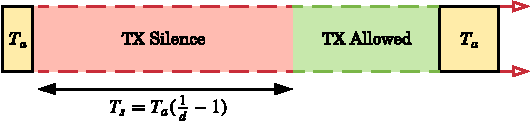
\includegraphics{Figures/duty_cycle_lorawan}
    \caption[\ac{lorawan} duty cycle enforcement]{
    Demonstration of how \ac{lorawan} enforces duty cycle limits; that is after a transmission of airtime $T_a$, the transmitter must be silent for a minimum period of $T_s=T_a(\frac{1}{d_c}-1)$ \cite{3YP:LIMITS_OF_LORAWAN}. The figure is to scale for $d_c=10\%$.
    }
    \label{fig:lorawan_duty_cycles}
\end{figure}

% Route management is the most researched challenge when it comes to ad-hoc networks \cite{3YP:MANET_RESEARCH_TRENDS} with implementations typically falling into the proactive or reactive categories - though more scenario specific variations do exist (e.g. geographic). Nodes using a proactive approach maintain a routing table for the whole network, to achieve this they rely on periodic updates from other nodes with their routing tables; these methods have low transmission delay but high ongoing overhead and adapt slowly to network changes. Nodes using a reactive approach explore the network when necessary to find a path, often by flooding route request packets; these methods have high transmission delay, but no ongoing overhead and can adapt to network changes immediately. Routing is not considered further in this paper so this is the abstracted level to which algorithms are considered. Full descriptions of many examples, including \ac{aodv} (reactive), \ac{olsr} (proactive) and \ac{lar} (geographic) can be found in \cite{3YP:ROUTING_ALGORITHMS}.







% ADR


 %https://www.ecodocdb.dk/download/25c41779-cd6e/Rec7003.pdf

%https://www.semtech.com/uploads/documents/etsi-compliance-sx1272-lora-modem.pdf



% Mesh (Ad-Hoc)

\chapter{\ac{lora} \ac{phy} Testing}
\section{Overview}
It has been repeatedly shown that \ac{lora} transmissions can be received at distances exceeding 10km in  unobstructed environments (free-space) when antennas are highly elevated \cite{3YP:LORA_RANGE_REVIEW}. However, these ideal radio conditions are not realistic for swarm robots operating in high-propagation environments such as forests. Therefore the first experiment in this paper attempts to identify the physical performance of \ac{lora} for the sparse swarm use case. 

\chapter{Testing  Platform}\label{sec:testing_platform}
\section{Hardware}
The basis of the designed test platform is HopeRF's\footnote{HopeRF Microelectronics Co. Ltd, China, https://www.hoperf.com/} RFM95W - a packet radio containing a \ac{lora} transceiver design licensed from Semtech; specifically, a broken out version from  Adafruit's\footnote{Adafruit, USA, https://www.adafruit.com/} is used. As a raw packet radio it provides direct access to the radio interface. An omni-directional 3dBi gain half-wavelength whip antenna is connected to the radio using a soldered uFL connector and a SMA to uFL connector. The net gain is assumed to be approximately 0dBm, after accounting for 1.5dBm loss in the cable (datasheet), 0.5dBm lost in the uFL connector (datasheet) and 1dBm lost through soldering (estimate). It is controlled by a Teensy\footnote{Teensy, https://www.pjrc.com/teensy/} 3.6 micro-controller, which also handles all logging responsibilities. A simple breakout circuit is implemented on strip-board to connect the components in a condensed package. Each breakout board features: a JST-PH2 battery connector, a coin cell holder for the Teensy's real-time-clock (\ac{rtc}), a power switch, a two-mode software switch, and three status LEDs. The schematic can be viewed in Figure \ref{fig:datalogger_schematic}. This is packaged to fit in an IP67 rated container with an internal lithium-polymer battery. Switches and SMA antenna connectors are external; these are IP67 rated and sealant is added where appropriate. The Teensy is equipped with an SD card for storage but, due to cost considerations, a GPS module is not implemented. A full breakdown of materials is listed in Figure \ref{fig:datalogger_cost}. The created test platforms, seen in Figure \ref{fig:dataloggers}, achieve the target of being a \ac{lora} datalogger suitable for all-weather.

\begin{figure}[H]
    \centering
    \begin{tabular}{cc}
    \subfloat[]{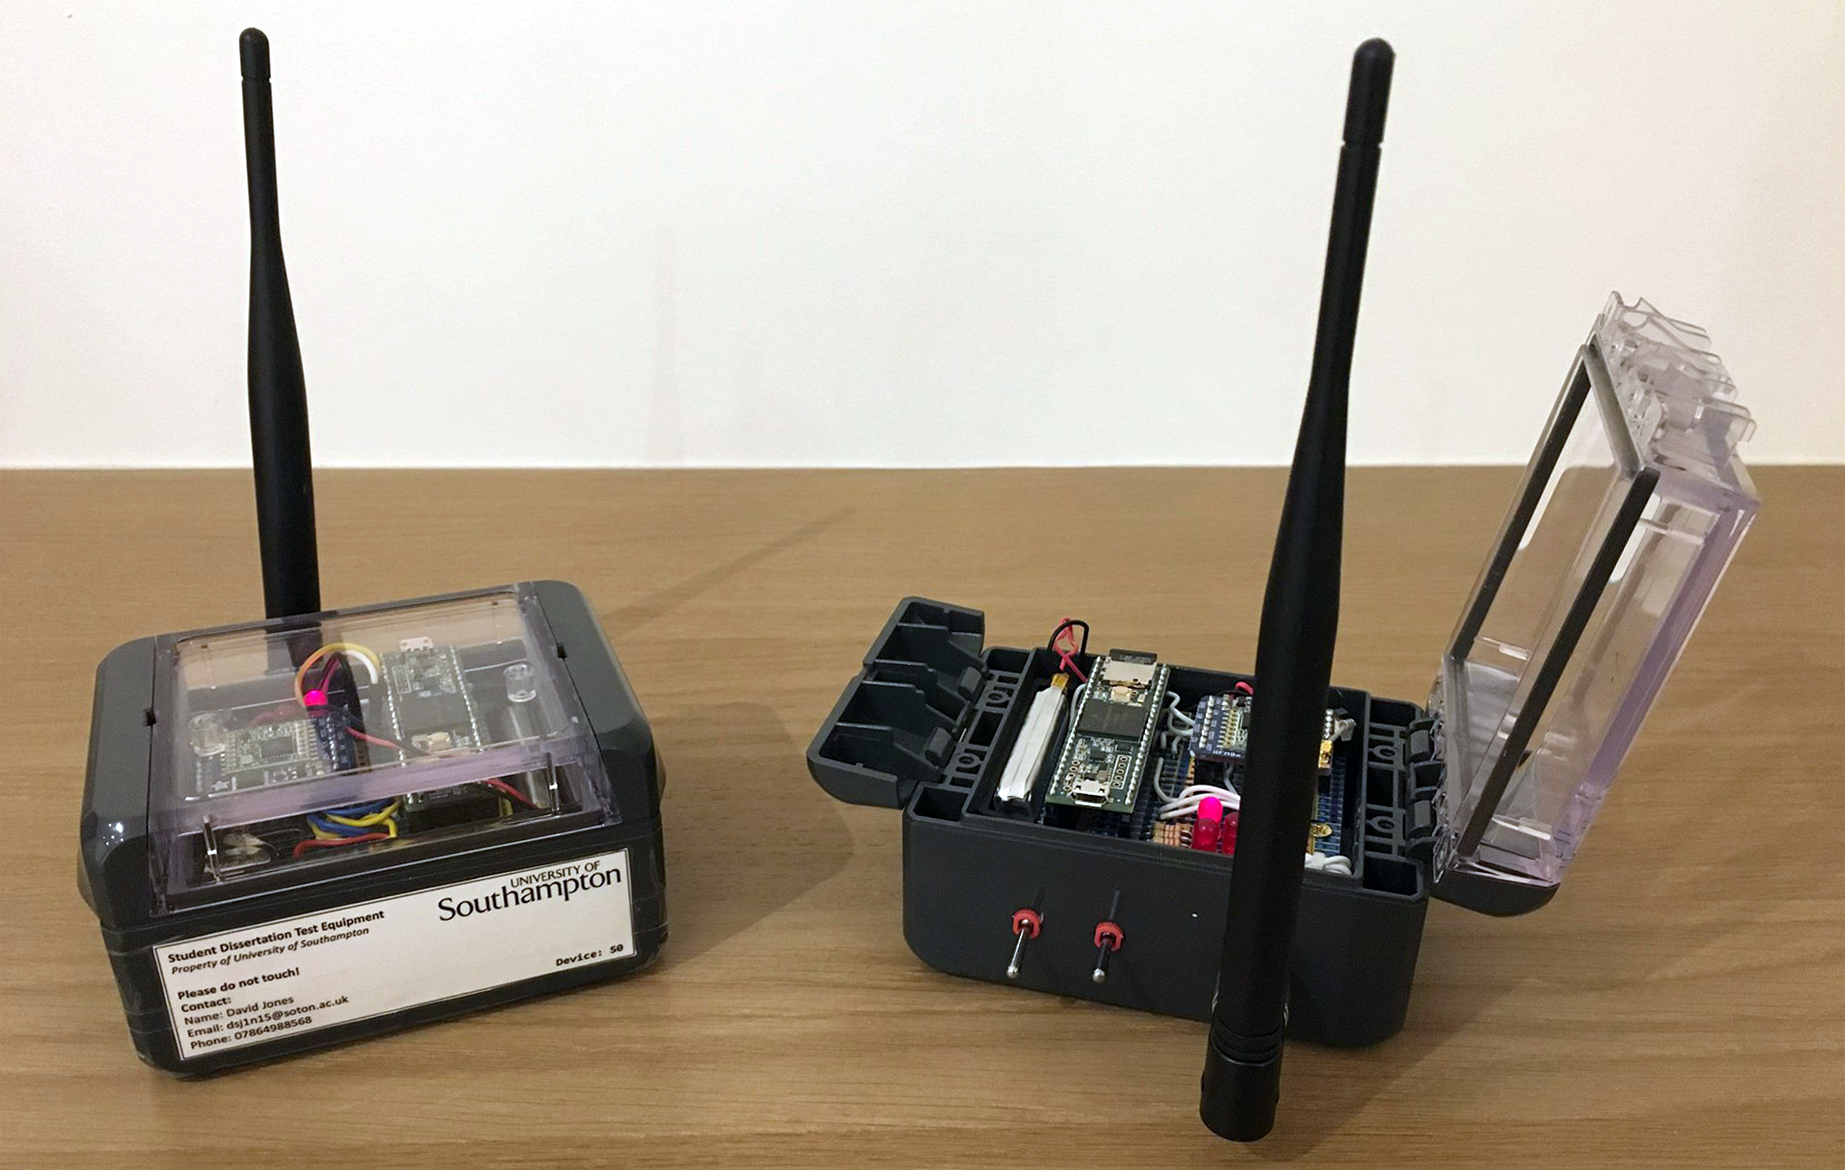
\includegraphics[height=5cm]{Figures/dl_both_devices.png}}
    \hspace{2.5mm}
    \subfloat[]{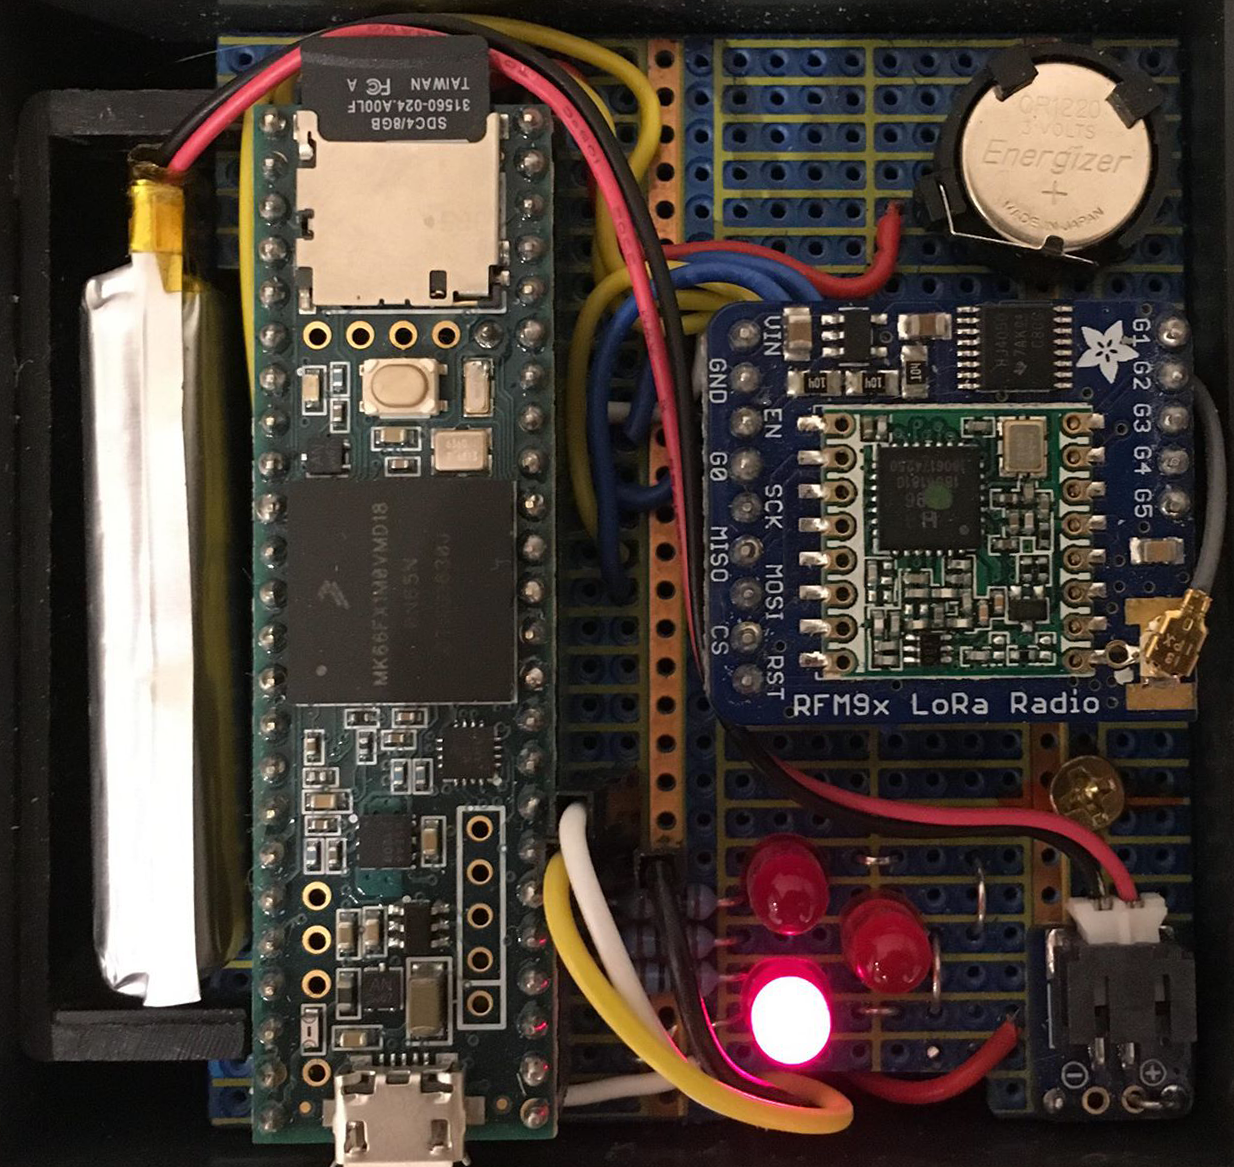
\includegraphics[height=5cm]{Figures/dl_circuit.png}}
    \end{tabular}
    \caption[Assembled testing platform]{External view of \texttt{S0} and \texttt{M0} platforms (left). Circuit view of \texttt{S0} (right); this is fixed into the assembly to avoid movement between tests. }
    \label{fig:dataloggers}
\end{figure}

\section{Software}\label{sec:test_platform_software}
The system is designed such that one device (a slave), can be left unattended at a fixed location and controlled by a second device (a master); this is achieved using a command control system, as explained in Figure \ref{fig:software_cmd_system}. Two command classes are defined for testing purposes; these are as follows:
\begin{itemize}
\vspace{-5mm}
	\item {\textbf{\texttt{HB\_CMD}}} : Command to trigger simple heartbeat functionality. When a slave receives this command it sends a heartbeat response (\textbf{\texttt{HB\_RSP}}) on the base configuration.
	\item {\textbf{\texttt{TD\_CMD}}} : Command to trigger execution of a test definition (\ac{td}). A \ac{td} holds a \ac{lora} configuration (values for \ac{cf}, \ac{sf}, \ac{tp}, \ac{bw}, \ac{cr}, \ac{pl}), a required \ac{pc}, and packet length. Figure \ref{fig:software_testdef_execution} explains the full control flow in detail.
	\end{itemize}
	
Slaves always listen to handle incoming commands, whereas the master can be set into two modes:
\vspace{-5mm}
\begin{itemize}
	\item \textbf{Heartbeat:} Sends periodic \texttt{HB\_CMD} commands, alerts user accordingly for every received or missed \textbf{\texttt{HB\_RSP}}.
	\item {\textbf{Run \ac{td}s:} Loads all stored \ac{td}s and handles them sequentially using \textbf{\texttt{TD\_CMD}}s.}
\end{itemize}
Interfacing with the radio is handled by the RH\_RF95 driver from the Radiohead\footnote{Radiohead, https://www.airspayce.com/mikem/arduino/RadioHead/} library. Operation of the software is detailed in Appendix \ref{sec:user_manual}.

\begin{figure}[p]
    \centering
    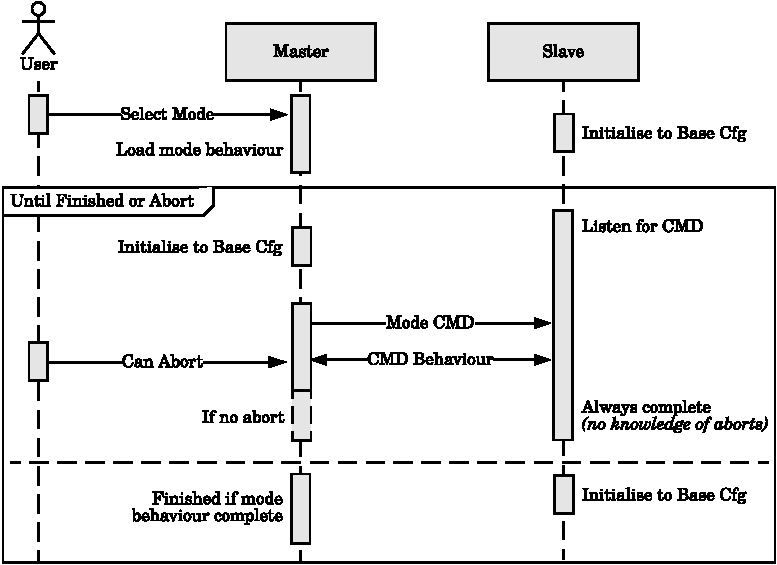
\includegraphics{Figures/software_cmd_system}
    \caption[Master-Slave command control method]{
    	Diagram showing master-slave command control method. Initially, both devices default to the same hardcoded radio parameters allowing two-way communication. This base state is chosen such that the expected range exceeds or matches that of the longest test range. When a mode is selected on the master, it sends the corresponding command to the listening slave and the behaviour is carried out. At any point the user may stop the master, and unless the slave is interacting with the master, it likely has no knowledge of this and will finish its behaviour. After command behaviour has finished the base configuration is reloaded in case it has been changed. In the case a master's mode requires multiple commands, the process repeats.
    }
    \label{fig:software_cmd_system}
\end{figure}
\begin{figure}[p]
    \centering
    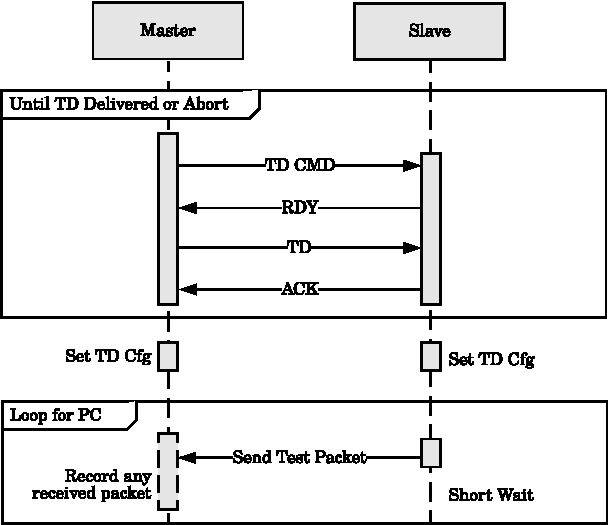
\includegraphics{Figures/software_testdef_execution}
    \caption[Master-Slave test definition execution method]{
    	Diagram showing execution of a single \ac{td}. After a \textbf{\texttt{TD\_CMD}} command is received, a short handshake takes place so that the master can share the \ac{td} to execute. After which both radios accordingly change their parameters and the slave sends the required \ac{pc}. Test packets are of length defined by the \ac{td} and contain a sequence identifier with the rest of data filled by a fixed data pattern. Any received packets are recorded along with \ac{rssi} and \ac{snr} values. Failed receives that occur due to bad CRCs are also recorded. This means that only transmissions where the preamble is not received are not recorded.
    }
    \label{fig:software_testdef_execution}
\end{figure}

\section{Methodology}
Simple testing scenarios devised.
so a phone was used for logging test coordinates manually

\section{Results}
\the\textwidth
\begin{figure}[H]
    \centering
   	\includegraphics{Figures/snr_pp_plot.eps}
    \caption[\ac{snr} vs packet percentage plot]{
    WRITE THIS DESCRIPTIONNN!!!
    }
    \label{master_slave_sequence}
\end{figure}

\subsection{Open (Free) Space}
High noise floor indicates that either the receiver's noise figure is not correct or there is more noise than expected in the environment. The fact that demodulation limit is nowhere near the true limit for SF10 onwards suggests that the cheaper radio does not perform correctly.


\subsection{Forest}
\subsection{Radio Height}

% Testing platform
% Testing methodology 
% Distance in relatively open space (got)
% Distance in trees (got)
% Closeness to ground (got)
% Coding rate ??? (sort of got)
% Difference in slight movements (!!!)
%Lessons Learnt 
https://www.thethingsnetwork.org/forum/t/no-lower-rssi-than-121-dbm-possible-in-ttn/19890/15
\chapter{MAC Protocol}
\section{The Problem}
There are t
A naive approach to message passing in a network will 


% Protocols based on transmission schedules    collision-free 
%  resource-inefficient 
%  may require well synchronized nodes throughout the network    difficult to adapt to changing topologies 
%Fundamentals of Wireless Sensor Networks: Theory and Practice Waltenegus Dargie and Christian Poellabauer © 2010 John Wiley & Sons Ltd.
%127 
%        Summary
%  Protocols that let nodes compete for access to the medium 
%  more flexible (easily accommodate changing network topologies)    require less overhead 
%  not collision-free 
%  must possess features that allow them to recover from collisions     network utilization may suffer when collisions occur frequently 


Provided that all nodes are within range of one another, with the use of \ac{cad} before transmissions, and ensuring that transmissions do not occur when a transmitter already has synchronisation \cite{3YP:LORA_SX12}, the vulnerable transmission collision period is very short. In fact collisions should only occur if \ac{cad}s of two transmitters overlap. Unfortunately, it is clear from \ac{phy} testing that for sparse scenarios, whether the environment has high propagation or not, \ac{lora} cannot deliver the required performance to achieve full coverage. This leads to the requirement of handling multi-hop communications and mitigating collisions due to the hidden node problem (highlighted in Figure \ref{fig:hidden_node_problem}).

Mobile-LMAC is a time division approach that can adapt transmission slots dynamically, however there is no mechanism to adjust 

 that would allow all robots to be within a single hop of one another. 


This leads to the requirement of multi-hop communications and handling of the significant challenges they present, namely: collisions (Section \ref{sec:lora_considerations}) in the presence of the hidden node problem (highlighted in Figure \ref{fig:collisions}) and routing (Section \ref{sec:adhocnetworks}). 


Uses Demand Assigned Multiple Access, relies on the fact that there are many channels and low probability of getting the same band, low spreading factors keep localisation where possible, and avoid conflicts with high spreading factor long range transmissions.

First check band that you're going to send in
Use knowledge of who is around from regular broadcasts on 1 band
Send out broadcast with slots for people to reply with CTR on other band (clear to receive)
Send out ATT (about to transmit)
Switch to lower sf and other band




%The \ac{csma} methods introduced in Section are unable to avoid all collisions in a multi-hop network due to the hidden node problem highlighted in Figure .



Can use any RTS, CTS layer
LoRa packets are limited to 255 bytes, but as shown by PHY testing, the shorter the packet, the more reliable it is.
Unable to exploit use of spreading factors as agreement must be made to change settings globally

%Unfortunately, CA does not effectively avoid all collisions in a multi-hop network. In the first place it is not usable when broadcasting, and so it cannot be used, for example, to improve traditional flooding broadcasting. In addition, the interference range of a node is usually greater than its trans- mission range. Specifically, a radio receiver can only decode a signal if the signal power exceeds a minimum threshold, and if the signal power is at least a given factor greater than the noise or interference power. Assume an intended receiver sends a CTS to ask all its neighbors to remain quiet during the upcoming transmission. A node that is just out of range of this receiver does not decode it, and is unaware that a transmission is in progress, and so proceeds to transmit its own packet. Although the node is too distant to directly communicate with the receiver, the strength of its trans- mission (which is noise to the receiver, which is listening to a different packet) may reduce the signal-to-noise ratio at the receiver enough that the receiver is unable to decode its incoming packet. Although it is a matter of semantics whether this should be classified as interference or collision, it is clear that even for unicast transmission CA does not always prevent one node’s communication from interfering with communication among other nodes.




When always within range the 
but also identifies a significant collision challenge caused by standard ALOHA protocols. THe 

Better to keep low duty cycle, 10\% will have massive collisions
From PHY testing it is known that 
Also know that if devics are moving, LOS changes in forests may suddenly cause packet failure, better to shove all data asap
 
Use 11, 9, 8, 7
Collision avoidance using channel sensing (e.g. via \ac{cad})

This will be extremely prevalent if there is a high 

By not focusing on power reduction, the high number of packets of adr is not requied.

single hop behaviour would no


Based on the physical performance in the environment about radio behaviour and imposed constraints from the theroetical about the technology  

Mainly target the local broadcast idea introduced in the introduction
Also consider how it can be adapted to  the other scenarios


It is unreasonable to expect 
% Coping with hops, on demand (reactive) or table driven (proactive), (minimise need but use AODV or DSR). 
%LoRa packets can only be 256 bytes (due to FIFO buffer size, see official documentation https://www.semtech.com/products/wireless-rf/lora-transceivers/SX1276).
%LoRa packet transmit time ranges from 200ms to 1s depending on packet size.\
%https://github.com/sudomesh/disaster-radio/wiki/Protocol
\section{Proposal}

Phy testing has shown that distance cannot be covered by a gateway
Proposed solution is agnostic to routing protocol

% Duty cycles (decided on method [manage per hour])
% Bands (dual band)
% Message types
% PHY layer parameter selection
% Adaptiveness???
% a461331.pdf general collision avoidance
%


 


% have robot knowing whos around from frequent packet updates
% robot can then decide on sending parameters before sending request

\section{Duty Cycle}
\begin{figure}[H]
    \centering
   	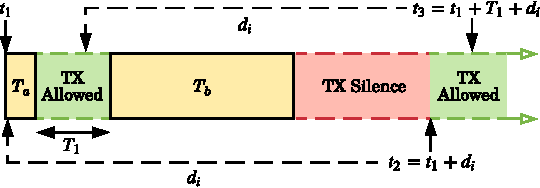
\includegraphics{Figures/duty_cycle_proposed.pdf}
    \caption[Proposed duty cycle enforcement method]{
    Demonstration of proposed method for duty cycle limit enforcement. Unlike \ac{lorawan}'s method the behaviour can vary greatly depending on when transmissions occur and how long they are, therefore this diagram is only a partial representation. It is valid provided there are no transmissions since $t=t_1-d_i$, where $d_i$ is the duty cycle interval (e.g. 3600 seconds). The duty cycle ($d_c$) shown is $\frac{T_a + T_b}{d_i}$. Enforcement is handled as follows. Immediately after the first transmission occurs, the remaining interval allowance is $T_b$ ($T_a+T_b-T_a$). This could be used immediately but, for purposes of demonstration, a short period of silence occurs. Once the transmission of length $T_b$ occurs, the remaining interval allowance is 0 ($T_b - T_b$), therefore the transmitter must be silent until allowance is freed. At $t_2$ a transmission of length $T_a$ would be allowed because for every time unit of a new transmission, the corresponding time unit of $T_a$ would no longer fall in the time interval. A longer transmission would not be allowed until $t_3$ because $T_b$ will not fall outside of the time interval until $T_1$ has elapsed. Note that as $T_a$ is already available the transmission can start $T_a$ before $T_b$ actually falls out of the interval. Therefore at $t_3$ a transmission of $T_a + T_b$ would be allowed (in this case, the full interval limit). The figure is not to scale.    
    }
    \label{fig:proposed_duty_cycle}
\end{figure}



Duty cycle:
Can quickly get complicated to understand when dealing with more complex transmission scenarios  (e.g. short send, wait, short send, wait, long send, etc...). However, simple to implement using a linked list, which gets culled when a send needs to occur. Delete old entries and find overlaps with current time - di. Can start sending as soon as the previous transmission started. Though processing intensive, allows predictable scheduling.


\chapter{Protocol Testing}
\section{Methodology}
Network simulations allow early assessment of basic protocol performance in controlled environments. Off-the-shelve simulation tools, such as ns-3\footnote{ns-3, https://www.nsnam.org}, offer very broad feature sets but consequently, creating an implementation with novel features, such as those present with \ac{lora} (\ac{cad}, orthogonal \ac{sf}s), is not trivial. Therefore, it was deemed more time-effective to create a specialised ad-hoc \ac{lora} simulator, using models from the \ac{phy} testing, with a subset of features relevant to the testing scenarios. The created simulator is detailed in the next section. The non-interface mode was used for gathering statistical results. Whereas, the GUI overlay was used for visually identifying node behaviour to aid understanding of statistical test results.
For each 
As the target of 
\% of intended recipients received for each message
Reasoning for failed receive: Insufficient SNR (out of range), CRC fail (bad luck), Sync Collision/ CRC from interference

Protocol 

The protocol 
Total helpful throughput number of bytes,  number of packets




Verification of the protocol is to be gauged on 
% Criteria of goodness is: 
 - \% of wanted packets received
 - \% of wanted bytes received
 - Total bytes received
 - Total packets delivered
 - Number of collisions on wanted messages

\chapter{\ac{lora} Ad-Hoc Simulator}
With an understanding of \ac{lora}'s performance - the next stage is to understand how \ac{lora} performs in an ad-hoc network. This section proposes a specialised Ad-Hoc \ac{lora} simulator, using models directly from \ac{phy} testing, as well as literature. It supports both scripted access for repeatable statistical testing and provides a GUI overlay for visually identifying system behaviour and performance. 

\textit{Full source code is available in the project design archive.}

\section{Model}
\subsection{Overview}
The model is considered as three main components, the environment, the radios, and time. The environment is responsible for understanding radio placement and the propagation channel between radios. Radios create new transmissions and poll the environment for existing transmissions, which they then attempt to receive. The simulator supports both the theoretical \ac{lora} radio (modelled from the datasheet), and the empirically defined RFM95W. Time progression of the system is modelled using the activity-oriented paradigm; this is where time is considered as small sequential slices at a selectable granularity (e.g. 1ms, 5ms, 10ms). For every simulation tick, the time-slice increments and any events that have occurred or are occurring within that time slice are handled. Unlike an event-driven approach, every time-slice is simulated, allowing for continuous receive behaviour close to that of a real-world scenario; the drawback being that it is processor intensive.


\subsection{Radio Model}
\subsubsection{Transmitting}
When a packet is transmitted, it is modelled in terms of start time, airtime and emanating location. Each time-slice the environment will poll each radio to collate all ongoing transmissions in the environment; this is the list which radios attempt to receive from and interference models are calculated for. If a radio's location changes between time-slices, the emanating location will be re-evaluated each time, however, the Doppler effect is not modelled because it has little effect for  on \ac{lora} at expected movement speeds \cite{3YP:DOPLER_EFFECT}. Transmission airtimes are calculated using the equations detailed in Section \ref{sec:airtime}.

\subsubsection{Receiving}
Every time-slice, a radio, provided it is not transmitting, will fill its receive buffer with a partial receive of the strongest receivable transmission (highest \ac{snr}) in the environment. For \ac{lora} transmissions, receivable implies the same \ac{sf}, \ac{bw} and \ac{cf} values are used. If multiple receivable signals are present, and the radio is not synchronised with a signal, the strongest will be captured. A small advantage is provided to favour receiving synchronised transmissions to support Class B and C collision scenarios. Class E collisions are handled by randomly adjusting receive \ac{snr}s slightly so that no preference is made between two signals with similar strength. Simulator collision results, as verified by the \texttt{TestCollision} class, are seen in Table  \ref{tab:sim_collisions}.

\begin{table}[H]
\centering\small
\caption[Simulator results for collision scenarios]{Results for collision scenarios defined in Table \ref{tab:collisions}, when modelled in the simulator. All scenarios are modelled correctly for all \ac{sf}s.}
\begin{tabular}{c|cc|c|c}
    \toprule
    \textbf{ID} & \textbf{Time} & \textbf{Power} & \textbf{Status} & \textbf{Metadata Status}\\
    \midrule\addlinespace
    A & $B_{start} > A_{\text{IP}}$ & $A_{\text{\ac{rps}}} \geq B_{\text{\ac{rps}}}$ & Receive A &  \cellcolor{green!25}\texttt{SUCCESS} \\
    B & $B_{start} > A_{\text{IP}}$ & $A_{\text{\ac{rps}}} < B_{\text{\ac{rps}}}$ & Receive A &  \cellcolor{green!25}\texttt{SUCCESS} \\
    C & $B_{start} > A_{\text{IP}}$ & $A_{\text{\ac{rps}}} \ll B_{\text{\ac{rps}}}$& CRC Fail A &  \cellcolor{green!25}\texttt{PAYLOAD\_COLLISION}  \\
    D & $B_{start}$ \textit{inside} $A_{\text{IP}}$ & $A_{\text{\ac{rps}}} \leq B_{\text{\ac{rps}}}$ & Collision &  \cellcolor{green!25}\texttt{PREAMBLE\_COLLISION} \\
    E & $B_{\text{IP}} \approx A_{\text{IP}}$ & $A_{\text{\ac{rps}}} \approx B_{\text{\ac{rps}}}$ & Collision &  \cellcolor{green!25}\texttt{PAYLOAD\_COLLISION}  \\
    F & $B_{\text{IP}} \approx A_{\text{IP}}$ & $A_{\text{\ac{rps}}} \gg B_{\text{\ac{rps}}}$ & Receive A &  \cellcolor{green!25}\texttt{SUCCESS} \\
    \addlinespace\bottomrule
\end{tabular}
\label{tab:sim_collisions}
\end{table}

Synchronisation is achieved when the important preamble of a signal (last 6.25 symbols) is in the receive buffer and demodulated successfully. Attempted demodulation occurs at the end of each time-slice and must pass at three stages to successfully receive a signal. If any stage fails the latter stages will not occur, but the signal will be unreceivable and may still interfere. The stages are:
\vspace{-2mm}
\begin{enumerate}[label=\textbf{S\arabic*}]
  	\item {When a transmission's first important preamble symbol is seen.	 \\Start of synchronisation.} \label{demod_s1}
  	\item {At the end of the transmission's preamble. At this point the radio is synchronised with a signal and is aware that it is receiving \cite{3YP:LORA_SX12}.} \label{demod_s2} 
  	\item {At the end of the transmission. Check for successful receive.} \label{demod_s3} 
\end{enumerate}
\vspace{-2mm}

\ref{demod_s1} purely checks if the signal is strong enough using the radio's demodulation curve. Failure will result in \texttt{NO\_PREAMBLE}, indicating a weak preamble. \ref{demod_s2} and \ref{demod_s3} also verify that enough of the transmission is present. This is required because it is possible that another powerful transmission has started filling the receive buffer - at this stage other signals are considered interference. For \ref{demod_s2}, 80\% of the signal must be preamble from the correct signal. For \ref{demod_s3} the amount of interference must not exceed the \ac{cr}'s capability (Table \ref{cr_effect}); this resembles burst-interference disrupting a portion of the signal. Failure due to interference will result in a \texttt{PREAMBLE\_COLLISION} or a \texttt{PAYLOAD\_COLLISION} for \ref{demod_s2} and \ref{demod_s3} respectively. Likewise a demodulation failure will result in either \texttt{NO\_PREAMBLE} or \texttt{WEAK\_PAYLOAD}. These statuses are simulation metadata, the radio does not necessarily know the failure details or that it even occurred - a mapping of metadata to radio knowledge is seen in Table \ref{tab:sim_metadata_translation}.

\begin{table}[H]
\centering\small
\caption[Simulator metadata to radio status mappings]{Mappings of simulator receive statuses to those the radio would see.}
\begin{tabular}{c|cc}
    \toprule
    \textbf{Metadata Status} & \textbf{Radio Status} & \textbf{Radio Aware} \\
    \midrule\addlinespace
	\texttt{NO\_PREAMBLE} & N/A & No \\
	\texttt{PREAMBLE\_COLLISION} & Collision & Yes \\
	\texttt{WEAK\_PAYLOAD} & \ac{crc} Fail & Yes \\
	\texttt{PAYLOAD\_COLLISION} & \ac{crc} Fail & Yes \\
	\texttt{SUCCESS} & Receive & Yes \\
    \addlinespace\bottomrule
\end{tabular}
\label{tab:sim_metadata_translation}
\end{table}

The mentioned demodulation curve varies depending on whether the theoretical model or the empirical RFM95W is used; only the latter is considered here. The transmission strength is calculated as the log-mean \ac{snr} of all its partial receives. The corresponding $p=\text{\ac{prp}}_{\text{\ac{snr}}}^{\text{\ac{sf}}}$ is found from the the best-fit sigmoid. If the \ac{snr} is close to $D_L$, $p$ is randomly adjusted to emulate high-variance behaviour. Demodulation success is then determined as a random chance with success $p$. The demodulation curves for receives at various \ac{snr}s are plotted in Figure \ref{fig:sf_sim_plot} (output generated by \texttt{FreeSpacePlot} class).

\begin{figure}[H]
    \centering
   	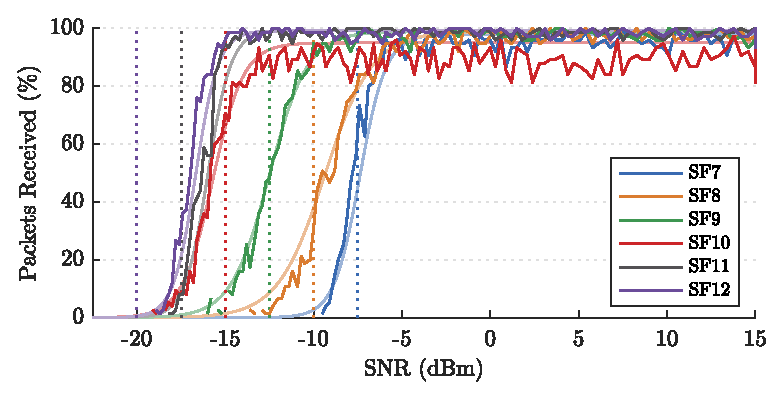
\includegraphics{Figures/sf_sim_plot}
    \caption[Simulator demodulation performance]{
    	Simulator demodulation performance, assessed as \ac{prp} for increasing \ac{snr}. Each point is the result of 75 transmitted packets at the respective \ac{snr}. The faded lines indicate the empirical fit curves from Section \ref{sec:demodulation_performance}. 
    }
    \label{fig:sf_sim_plot}
\end{figure}

\subsubsection{CAD}
\ac{lora}'s \ac{cad} process requires the ability to poll the receive buffer for a preamble symbol. When the process is invoked, the initial contents of the receive buffer are emptied as previous receive data cannot be used. A symbol's length of receive buffer is then captured (Equation \ref{eq:symbol_time}) and then the \ac{cad} search result is returned after the average processing time ($0.85\cdot S_T$) \cite{3YP:LORA_SX12}. Activity is detected if at least 80\% of the receives in the buffer are preamble symbols and a standard demodulation curve check passes. When the process is complete the full receive buffer is dumped as it cannot be used for receives.

\subsection{\ac{rps} ($R_P$) \& \ac{snr} Model}
The actual receivable signal power of a transmission is derived from the link budget equation, Equation \ref{eq:rp} explicitly repeats this for the factors modelled.
\begin{equation}
\label{eq:rp}
	R_P = TX_{power} + TX_{gain} + RX_{gain} - P_{loss}^{TX\rightarrow RX}
\end{equation}
Gains at the receiver and transmitter end are broken down into fixed antenna gains and cable losses. The path loss ($P_{loss}$) is broken down into free-space loss and object loss. A global free-space model is used for the environment, selectable at creation. Although adding any new model is straightforward,  built-in options include those defined in Section \ref{sec:environment_propagation}: E-FSPL, FSPL, PE. 

\begin{figure}[H]
    \centering
   	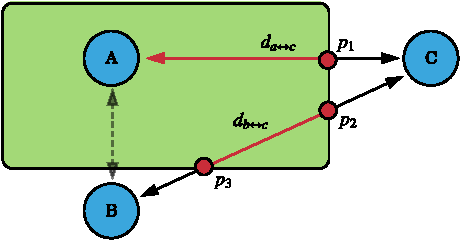
\includegraphics{Figures/obstacle_diagram}
    \caption[Object path loss scenarios]{
    	Scenarios for LOS path loss whilst passing through objects.   
    }
    \label{fig:object_path_loss}
\end{figure}

Objects are entities in the environment, which will possess their own propagation model; built-in models include: COST235, Weissberger and the ITU-R. Forests are a type of built-in object; these can take any 2D shape and use the ITU-R model with a $\beta$ multiplier. All this combined allows the path loss curves from Section \ref{sec:environment_propagation} to be recreated. Of course in a real environment, it is likely that not all radio transmissions will pass through the same obstacles. There is no perfect way to handle this, the closest would be the one woodland terminal model \cite{3YP:RF_BOOK} but this sets severe limits; one radio must be in the object and the other outside with no other obstacles in the path. Therefore a more approximate approach is taken. In short the total $P_{loss}$ is sum of the free-space loss and the segment of the propagation curve from the obstacle.  Using Figure \ref{fig:object_path_loss} as a scenario reference, the following are examples of extra $P_{loss}$ due to obstacles. Equation \ref{eq:path_loss_a_c} calculates for $A\leftrightarrow C$ where one radio is in the obstacle.
    	\begin{equation}
    	\label{eq:path_loss_a_c}
    	\begin{split}
    	    	P_{loss \text{ (Object)}}^{A\rightarrow C} = P_{loss}^{A\rightarrow p_1}
    	\end{split}
    	\quad\leftrightarrow\quad
    	\begin{split}
    		    P_{loss \text{ (Object)}}^{C\rightarrow A} = P_{loss}^{C\rightarrow A}-P_{loss}^{C\rightarrow p_1}
    	\end{split}
    	\end{equation}
    	Equation \ref{eq:path_loss_b_c} calculates for $B\leftrightarrow C$ where the transmission completely passes through the object.
    	\begin{equation}
    	\label{eq:path_loss_b_c}
    	\begin{split}
    	        P_{loss \text{ (Object)}}^{B\rightarrow C} = P_{loss}^{B\rightarrow p_2}-P_{loss}^{B\rightarrow p_3}	
    	\end{split}
    	\quad\leftrightarrow\quad
    	\begin{split}
    	    	P_{loss \text{ (Object)}}^{C\rightarrow B} = P_{loss}^{C\rightarrow p_3}-P_{loss}^{C\rightarrow p_2}
    	\end{split}
    	\end{equation}
    
    As the method has large swings in path loss depending on whether obstacles are close to the receiver or transmitter, $\text{max}(P_{loss}^{TX\rightarrow RX}, P_{loss}^{RX\rightarrow TX})$ is taken; this means path loss will be the same regardless of the transmission direction -- interference differences may still mean that \ac{snr} varies. The model scales to any number of objects in the path. Note that fast-fading is abstracted into the demodulation curve of the receiver and is not modelled separately.  	

The channel power as seen by a receiver (\ac{rssi}) at a location, is modelled as the sum of: all `interfering' signal powers, the thermal noise floor ($T_N$), and the receiver noise figure ($N_f$). When attempting to receive a signal, its observed $R_P$ can removed from the \ac{rssi} calculation to provide the channel noise ($N$). The \ac{snr} can then be calculated as $R_P - N$. Interfering sources, narrowband or otherwise, are considered as those where the bandwidth used overlaps with the receive channel. As per \ac{lora}'s orthogonality defined in Section \ref{sec:sf_orthogonality}, a \ac{lora} transmission is only considered to interfere if the chirp rate is the same as that of the receive configuration.


\subsection{Protocol Testing Infrastructure}
Protocols are implemented the layer above the low-level radio behaviour using a listener infrastructure. When the time-slice increments, first the raw radio behaviour will occur, and then a `tick' process will be called on any listeners. These listeners can maintain their own state between ticks allowing them to schedule transmissions and handle received packets, ultimately allowing emulation of a full protocol stack. More implementation specific behaviour like radio movement can be emulated here or on a higher level listener. This is how all the protocols defined in Section \ref{sec:protocols} are implemented. The base listener class, \texttt{ProtocolTickListener}, provides methods for directly handling events that have occurred the previous tick (synchronisations, receives, CAD results), tracks received data, and handles protocol performance tracking (for testing). Statistics can be dumped with a by-radio perspective -- the number of  packets received by each radio and the reason for any failures. Or with a by-transmission perspective -- the number of receivers of each transmission and the reason for any failures. Outputs can be filtered to disregard failures of transmissions that are not `wanted' by a receiver (see Section \ref{sec:mac_considerations}).

The execution of an environment (and the radios within it) is handled by an \texttt{EnvironmentRunner}; this can step time by the configured granularity a number of times or run continuously. Execution occurs on a separate thread and employs listeners to allow external interaction either through a test harness or GUI. Events can be created and scheduled for execution at fixed times to allow for scripted test behaviour; there is built-in support for moving radios, sending transmissions and verifying the expected radio state; although, with full control over the system, any custom behaviour can be implemented. 


\section{Interface (GUI)}
The Java Swing interface acts largely as a wrapper for managing an \texttt{Environment} \texttt{Runner} and displaying the environment being executed. The full interface can be seen in Figure \ref{fig:sim_interface_main} with further examples in Appendix \ref{sec:simulator_pictures}. User controls are provided for managing environment time, choosing presets and protocols, and accessing statistics. The graphical view, which has full support for panning and zooming, displays the environment's: objects, radios and transmissions. Objects are drawn using their obstruction shape (and specified attributes). Radios are blue circles when transmitting and grey otherwise. Transmission routes are displayed for the last received data in a radio's buffer as a line from transmitter to receiver with \ac{snr} indicated; preamble is identfied by a dotted line, payload as a solid line. The line will be grey if the receiver failed to synchronise with the preamble or red if the transmission was not the one the receiver is synchronised with. Otherwise, blue is used to indicate a data packet and orange as protocol overhead. Together visual cues provides an exact understanding of behaviour.

\begin{figure}[H]
    \centering
   	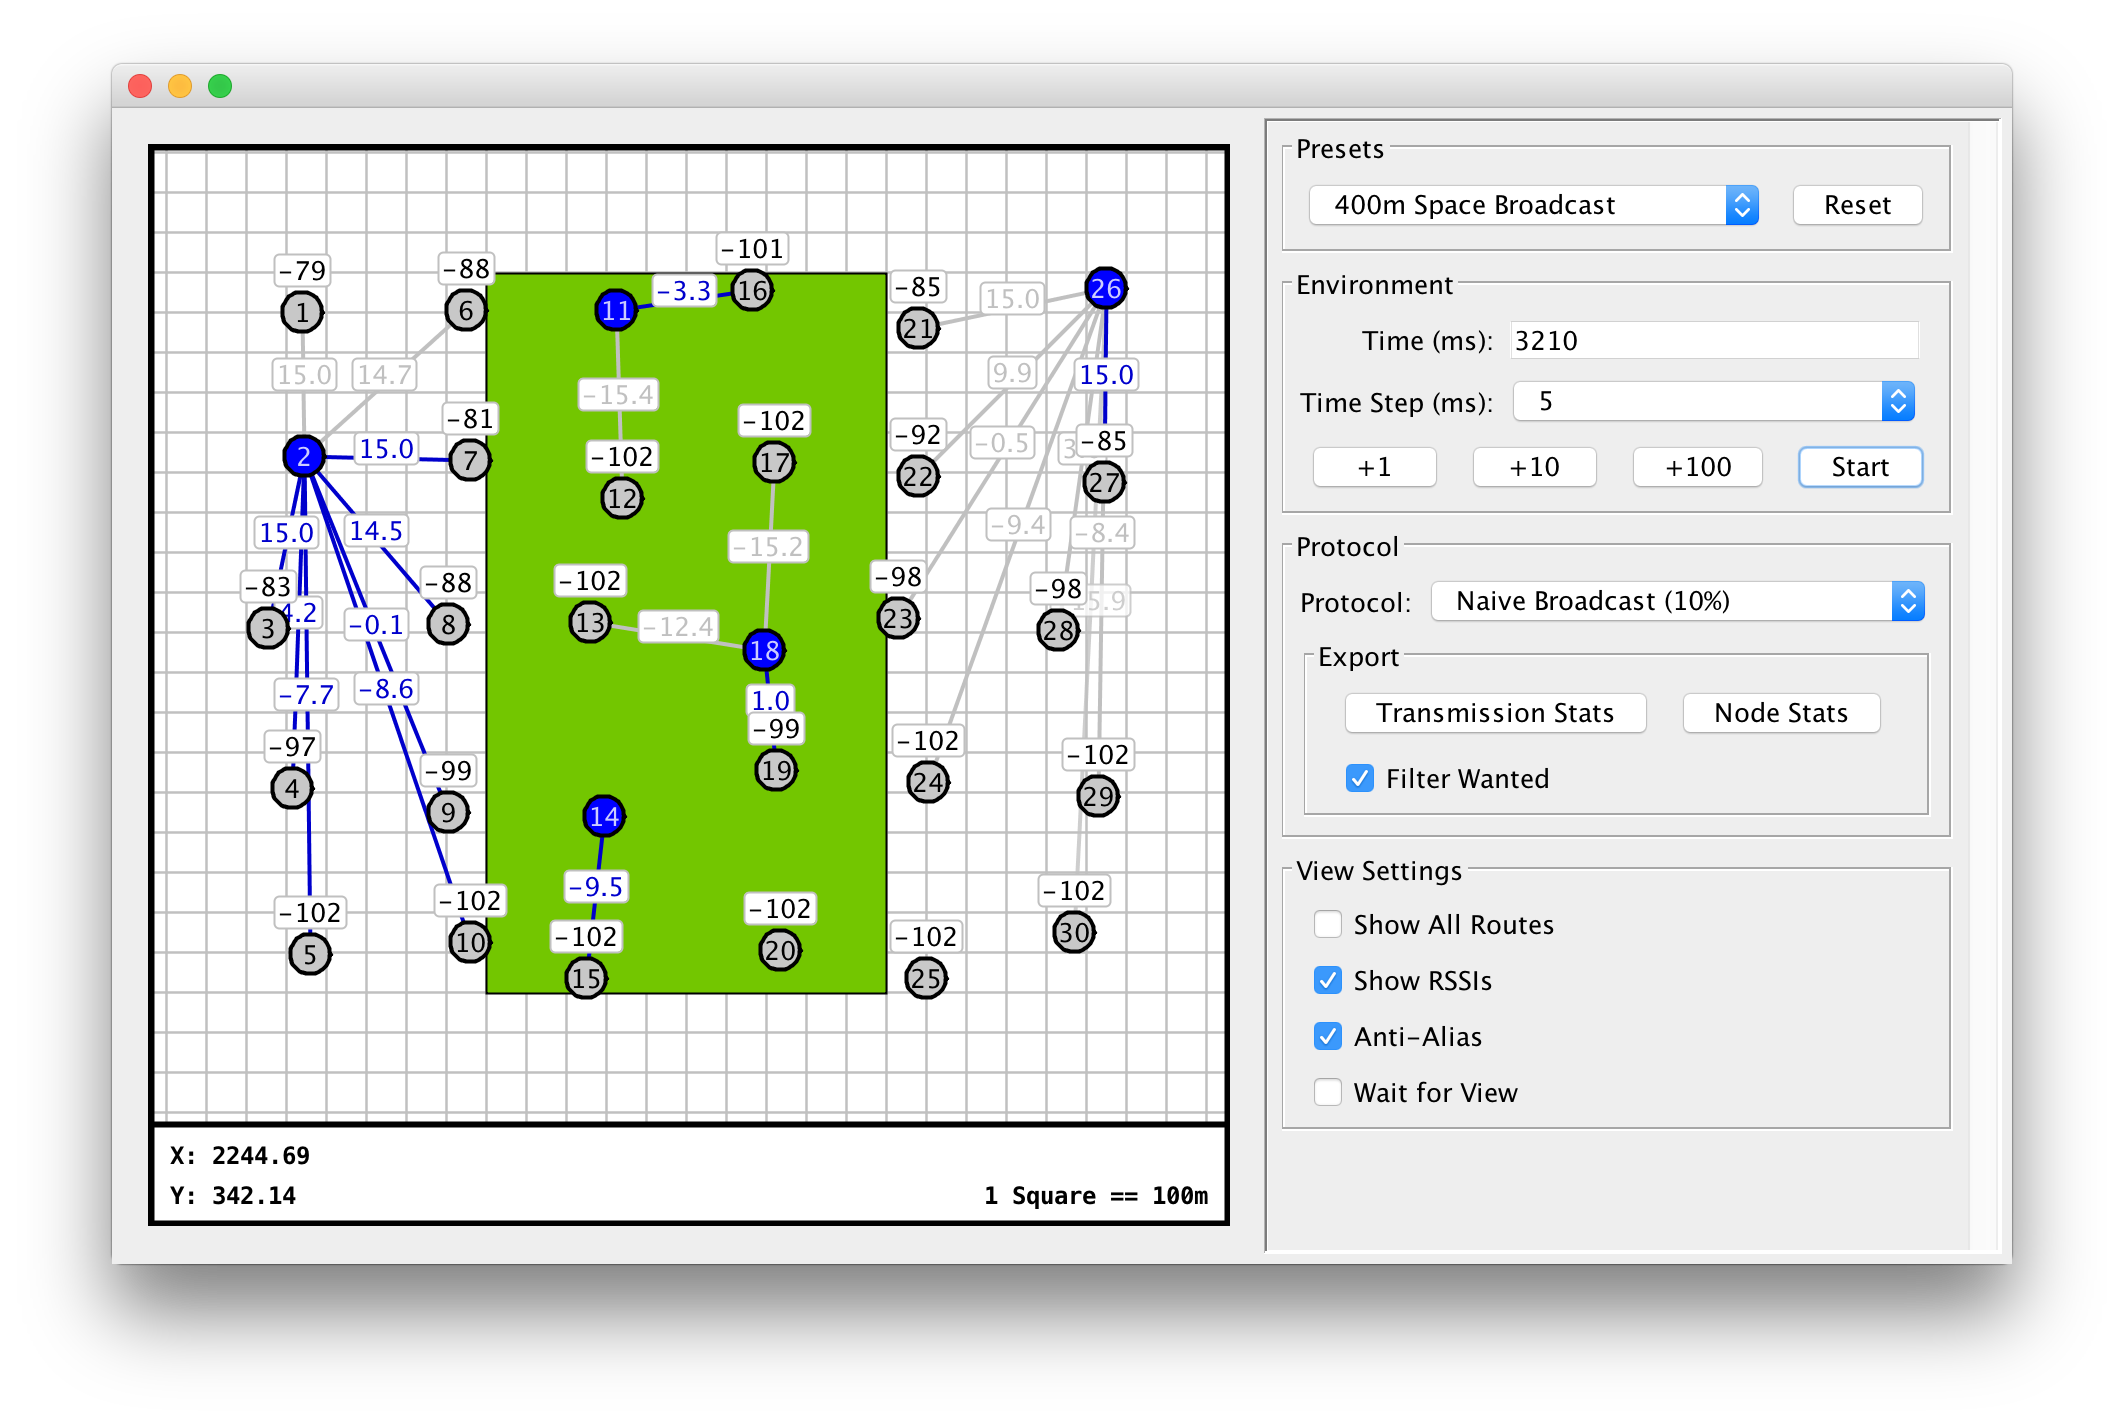
\includegraphics[width=\textwidth]{Figures/simulator_main}
    \caption[Simulator GUI example]{ 
    	Simulator's GUI interface running the naive (ALOHA) protocol.
    	}
    \label{fig:sim_interface_main}
\end{figure}





%Network simulations allow early assessment of basic protocol performance in controlled environments. Off-the-shelve simulation tools, such as ns-3\footnote{ns-3, https://www.nsnam.org}, offer very broad feature sets but consequently, creating an implementation with novel features, such as those present with \ac{lora} (\ac{cad}, orthogonal \ac{sf}s), is not trivial. Therefore, it was deemed more time-effective to create a specialised ad-hoc \ac{lora} simulator, using models from the \ac{phy} testing, with a subset of features relevant to the testing scenarios. The created simulator is detailed in the next section. The non-interface mode was used for gathering statistical results. Whereas, the GUI overlay was used for visually identifying node behaviour to aid understanding of statistical test results.
\section{Discussion}
Approaches suited to DTN





\chapter{Conclusion}
This paper has presented an assessment of \ac{lora} for sparse swarm scenarios covering: physical radio performance, regulation concessions, and how that maps to prospective \ac{mac} protocol performance. Conclusions are that \ac{lora}'s physical technology is suitable with recorded transmit ranges, using typical \ac{lora} radios, far exceeding that achievable by Wi-Fi or other comparable technologies -- 1600m in free-space or 500m in high-propagation forest can be expected even with scenario compromises. 

That being said, given its naturally low-data-rate, the technology is severely handicapped by Sub-1GHz band limitations in Europe. Future work could study the more freely regulated 2.4GHz \ac{lora} implementation, though this is unlikely to be applicable to forest scenarios. The usable unicast throughput of ${\sim}15\text{KB}$ per hour (${\sim}2.5\text{KB}$ if multiple channels are required),  whilst conforming to regulation is significantly worse than can be expected from usual swarm transfer mediums. LoRa's multiple data-rate configurations could alleviate this, either through manual configuration on a deployment basis, or through a \ac{mac} protocol. 

The attempts in this paper to create said protocol were ultimately unsuccessful, with basic ALOHA and \ac{csma} approaches outperforming the proposed \ac{llbp}. A variation on \ac{llbp} with slotting or minor tweaks may be able to deliver better/equal performance, or a contention-free Mobile-LMAC \cite{3YP:WSN_BOOK} like approach may be required. The potential of new cheaper gateway devices could help deliver a solution to this problem but this is all a topic for future research.

Though overall the created simulator provided a reasonable assessment of protocols and proposed some novel modelling techniques to closely emulate real-world context, one drawback of the testing approach was that decisions were made mostly agnostic to scenario data. Given \ac{mac} layers can be very scenario specific, implementing realistic swarm data models and distribution algorithms like SOUL \cite{3YP:SOUL} would give more relatable between-protocol assessment. The protocol may need to be fully integrated into a network stack, e.g. with routing protocols, for this. Ultimately, this should lead to real-world verification with radio hardware; the proposed logging platform would be suitable for this.



%\% of intended recipients received for each message
%Reasoning for failed receive: Insufficient SNR (out of range), CRC fail (bad luck), Sync Collision/ CRC from interference
%
%Missed == This implies the receiver was busy, busy receiving at the same time or not receivable 
%No Preamble on a Wanted == This implies the SF is not adequate
%
%The protocol 
%Total helpful throughput number of bytes,  number of packets

%One approach may be to slot transmissions so there is always a good time to send announcements. 
%A more complex method could require a handshake between receivers and broadcaster using slotted schedules, but this is high overhead and massively increases nearby death
%If it costs more to send out the 

%First check band that you're going to send in
%Use knowledge of who is around from regular broadcasts on 1 band
%Send out broadcast with slots for people to reply with CTR on other band (clear to receive)
%Send out ATT (about to transmit)
%Switch to lower sf and other band

%Unable to exploit use of spreading factors as agreement must be made to change settings globally

%From PHY testing it is known that 
%Also know that if devics are moving, LOS changes in forests may suddenly cause packet failure, better to shove all data asap
 

\chapter{Retrospective}
Ideally would have had rain data but data loggers messed up

A lot of work was put into the test platform software before changed to simulation

% 40 hours or so of on site data collection
% Lost time from trying to develop on hardware
% 


\printbibliography

\appendix
\chapter{Design Archive}
\begingroup
\raggedright\small
\definecolor{folderbg}{RGB}{124,166,198}
\definecolor{folderborder}{RGB}{110,144,169}
\newlength\Size
\setlength\Size{4pt}
\tikzset{%
  folder/.pic={%
    \filldraw [draw=folderborder, top color=folderbg!50, bottom color=folderbg] (-1.05*\Size,0.2\Size+5pt) rectangle ++(.75*\Size,-0.2\Size-5pt);
    \filldraw [draw=folderborder, top color=folderbg!50, bottom color=folderbg] (-1.15*\Size,-\Size) rectangle (1.15*\Size,\Size);
  },
  file/.pic={%
    \filldraw [draw=folderborder, top color=folderbg!5, bottom color=folderbg!10] (-\Size,.4*\Size+5pt) coordinate (a) |- (\Size,-1.2*\Size) coordinate (b) -- ++(0,1.6*\Size) coordinate (c) -- ++(-5pt,5pt) coordinate (d) -- cycle (d) |- (c) ;
  },
}
\forestset{%
  declare autowrapped toks={pic me}{},
  pic dir tree/.style={%
    for tree={%
      folder,
      font=\ttfamily,
      grow'=0,
    },
    before typesetting nodes={%
      for tree={%
        edge label+/.option={pic me},
      },
    },
  },
  pic me set/.code n args=2{%
    \forestset{%
      #1/.style={%
        inner xsep=2\Size,
        pic me={pic {#2}},
      }
    }
  },
  pic me set={directory}{folder},
  pic me set={file}{file},
}


Overview of folder structure in the design archive, not all low-level folders are indicated.\\
\vspace{5mm}

\begin{forest}
  pic dir tree,
  where level=0{}{
    directory,
  },
[design\_archive.zip, file
  [datalogger\_schematic
  ]
  [datalogger\_source
    [LoRa\_Datalogger
    ]
    [LoRa\_Board\_ID\_Setter
    ]
  ]
  [logged\_data
    [location\_pictures
  	]
  	[location\_results
  	]
  	[testdefs
  	]
  ]
  [processing\_scripts
  ]
  [simulator\_output\_data
  ]
  [simulator\_source
      [LoRa\_Simulator
    ]
  ]
]
\end{forest}

\textit{PlatformIO build files provided for datalogger source} \\
\textit{Maven POM (Project Object Model) file provided for building simulator.}

\textit{MATLAB scripts require the library functions \texttt{sigm\_fit}\footnote{\texttt{sigm\_fit.m}, rpavao@gmail.com, 2016}, \texttt{vline}/\texttt{hline}\footnote{\texttt{vline.m}/\texttt{hline.m}, Brandon Kuczenski, Kensington Labs, 2001} and \texttt{haversine}\footnote{\texttt{haversine.m}, Josiah Renfree, 2010}}
\endgroup




\chapter{Datalogger Schematic}
\begin{figure}[H]
    \centering
    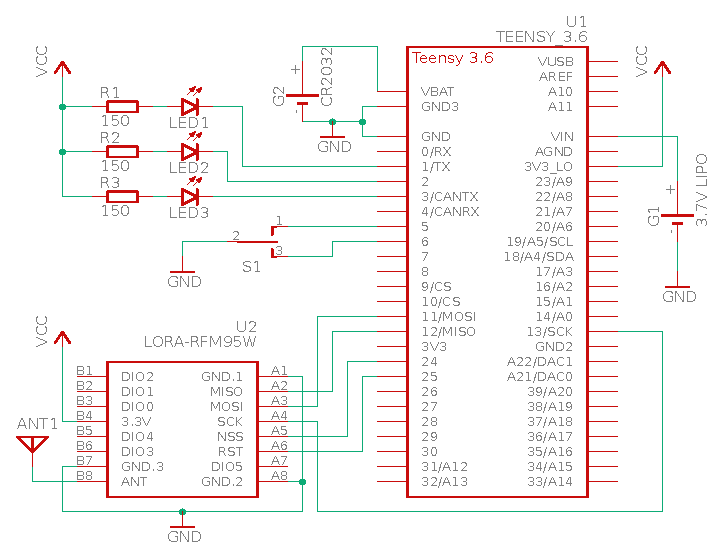
\includegraphics[width=\textwidth]{Figures/datalogger_schematic.eps}
    \caption[Datalogger schematic]{Autodesk EAGLE schematic for datalogger hardware.}
    \label{fig:datalogger_schematic}
\end{figure}

\chapter{Datalogger User Manual}\label{sec:user_manual}
\textbf{User Manual for Datalogger Software} \\ 
Firmware Version v1.0

\textbf{Overview}\\
The firmware in contained in the design archive, see \texttt{LoRa\_Datalogger}. The same firmware is used for Master and Slave devices to reduce the chance of inconsistent behaviour. The 8-bit board identifier, which is stored in Teensy EEPROM, is used to determine datalogger type. The top two bits are reserved, with B7 identifying a Master and B6 identifying a Slave, all other bits should be used to assign a unique identifier. A tool is provided in the design archive to set this appropriately, see \texttt{LoRa\_Board\_ID\_Setter}.

Full detail of master-slave commands and their purpose are included in Section \ref{sec:test_platform_software} of the main report; this manual is to instruct on how the software actually operates.

\textbf{Hardware}\\
The following hardware positions are for a device oriented such that the Teensy is on the left, the radio is on the right and the transparent top is facing upwards.

The status LEDs are as follows: \\
\phantom{-}\hspace{1cm}Bottom - \textbf{\texttt{LED\_1}} \\
\phantom{-}\hspace{1cm}Middle - \textbf{\texttt{LED\_2}}\\
\phantom{-}\hspace{1cm}Top - \textbf{\texttt{LED\_3}}

Switches are as follows: \\
\phantom{-}\hspace{1cm}Left - \textbf{\texttt{POWER\_SWITCH}} \\
\phantom{-}\hspace{1cm}Right - \textbf{\texttt{SOFTWARE\_SWITCH}}

\newpage\textbf{Common Power-On Behaviour}\\
All device types carry out the same boot sequence before device type specific behaviour, this is as follows:
\begin{enumerate}[label=\textbf{\arabic*}]
	\item  Before powering on the device, the \textbf{\texttt{SOFTWARE\_SWITCH}} can optionally be set to its bottom position to delay boot up until a serial monitor is attached to the Teensy USB. Other positions will boot up as normal. Waiting can be cancelled during boot-up by changing the switch back to any other position.
	\item Power on device by setting the \textbf{\texttt{POWER\_SWITCH}} to its bottom position. All other positions indicate off.
	\item \textbf{\texttt{LED\_1}}, \textbf{\texttt{LED\_2}} and \textbf{\texttt{LED\_3}} will turn on.
	\item The datalogger will initialise serial communications.
	\item \textbf{\texttt{LED\_3}} will turn off.
	\item The datalogger will sync with the real time clock (\ac{rtc}).
	\item The datalogger will check if it is a master or a slave using the board identifier stored in the EEPROM. If the identifier is not found or is invalid, the device will go into error state.
	\item The radio will initialise using the hardcoded configuration. On initialisation failure the device will go into error state.
	\item \textbf{\texttt{LED\_1}} will turn off.
	\item The SD card will initialise. If this is unsuccessful, boot-up will not fail but not all functionality may be available.
	\item If the \textbf{\texttt{SOFTWARE\_SWITCH}} switch is not in its middle position then boot-up will pause until it is.
	\item \textbf{\texttt{LED\_2}} will turn off.	
\end{enumerate}

When boot up is finished either \textbf{\texttt{LED\_1}} or \textbf{\texttt{LED\_3}} will be lit continuously indicating if the board is a Slave or Master respectively. If an error state is entered then \textbf{\texttt{LED\_2}} will flash continuously. The device must be rebooted to resolve this. It is suggested that a serial connection is connected before boot to discover any issues.

\newpage\textbf{Slave Behaviour}\\
Behaviour is dictated by \texttt{SOFTWARE\_SWITCH} position:
\vspace{-5mm}
\begin{itemize}
	\item \textbf{Bottom} : No Behaviour \textit{(Reserved)}
	\item \textbf{Middle} : Idle
	\item \textbf{Top} : Command Handling Mode
\end{itemize}
All modes use \textbf{\texttt{LED\_2}} to indicate a successful send or receive, and  \textbf{\texttt{LED\_1}} to indicate any failures. Behaviour can be cancelled at any time by returning the \texttt{SOFTWARE\_SWITCH} switch to the middle position.

\textbf{Master Behaviour}\\
During boot, if any of the following folders/files do not exist, they are created:
\vspace{-5mm}
 \begin{itemize}
 \item \texttt{/testdefs/} - Folder for placing test definitions.
 \item \texttt{/results/} - Folder that results are saved to.
 \item \texttt{/testdefs/\_format.txt} - File with current firmware's expected format for test definitions. As of v1.0 this is a file containing the following fields: \texttt{exp\_range,\\packet\_cnt,packet\_len,freq,sf,tx\_dbm,bw,cr4\_denom,preamble\_syms,crc,}\\ \textit{Note that the final comma is required, examples are provided in the design archive}
 \end{itemize}


Behaviour is dictated by \texttt{SOFTWARE\_SWITCH} position:
\vspace{-5mm}
\begin{itemize}
	\item \textbf{Bottom} : Heartbeat Mode. Sends continuous heartbeat commands, \textbf{\texttt{LED\_2}} will flash for a received response, \textbf{\texttt{LED\_1}} will flash for failure.
	\item \textbf{Middle} : Idle
	\item \textbf{Top} : Test Definition Mode. If the SD card is not present then this mode will not have any behaviour. Otherwise, all test definitions will be loaded and executed in order of expected range (longest range first). If no packets are received at a range level, the remaining test definitions are not executed. A test definition's results are stored in a single file, in a folder timestamped with the time the mode was executed. \textbf{\texttt{LED\_2}} indicates a test definition is being executed. \textbf{\texttt{LED\_1}} will flash on test definition delivery failure. All LEDs will be lit when the test finishes.
\end{itemize}
Behaviour of any mode can be cancelled at any time by returning the \texttt{SOFTWARE\_SWITCH} switch to the middle position.












% \chapter{Gantt Charts}

% Current work
\begin{figure}[H]
\centering
\begin{ganttchart}[vgrid, hgrid]{1}{14}
  \gantttitle{Week}{14} \\
  \gantttitlelist{1,...,14}{1} \\
\ganttbar{Project decision\ \ }{1}{2} \\
\ganttbar{Brief writing\ \ }{2}{2} \\
\ganttmilestone{Project Brief\ \ }{2} \\
\ganttlink{elem1}{elem2}
\ganttbar{Research\ \ }{3}{13} \\
\ganttbar{LoPy Testing\ \ }{3}{7} \\
\ganttbar{RFM95 Testing\ \ }{9}{10} \\
\ganttbar{Datalogger design\ \ }{11}{12} \\
\ganttlinkedbar{Datalogger construction\ \ }{12}{13} \\
\ganttbar{Interim report writing\ \ }{11}{13} \\
\ganttmilestone{Interim Report\ \ }{13} 
\ganttlink{elem8}{elem9}
\end{ganttchart}
\caption[Interim report Gantt chart]{Gantt chart for work up to interim report (week 13)}
\label{fig:past_gantt_chart}
\end{figure}
\newpage

% Planned work
\vspace*{\fill}
\begin{figure}[H]
\centering
\begin{ganttchart}[vgrid, hgrid]{1}{22}
  \gantttitle{Week}{22} \\
  \gantttitlelist{14,...,35}{1} \\
\ganttbar{Datalogger software\ \ }{1}{2} \\
\ganttlinkedbar{LoRa field testing\ \ }{2}{4}
\ganttbar{}{7}{8} \\
\ganttbar[bar/.append style={fill=red}]{Exam period\ \ }{5}{6} \\
\ganttlink{elem3}{elem2}
\ganttlinkedbar{Data analysis\ \ }{8}{10} \\
\ganttbar{Simulator development\ \ }{9}{11} \\
\ganttbar{Protocol development\ \ }{11}{17} \\
\ganttbar{Protocol analysis\ \ }{13}{17} \\
\ganttbar{Protocol field testing\ \ }{18}{19} \\
\ganttbar{Final report writing\ \ }{16}{21} \\
% Second
\ganttmilestone{Final Report\ \ }{21} 
\ganttlink{elem9}{elem10}
\end{ganttchart}
\caption[Planned progress Gantt chart]{Planned Gantt chart for work from interim report hand-in (week 13) up until hand-in of final report. Red indicates periods where no work completion was expected.}
\label{fig:planned_gantt_chart}
\end{figure}
\vspace*{\fill}
\newpage

% Actual work
\vspace*{\fill}
\begin{figure}[H]
\centering
\begin{ganttchart}[vgrid, hgrid]{1}{21}
  \gantttitle{Week}{21} \\
  \gantttitlelist{14,...,34}{1} \\
\ganttbar{Datalogger Software\ \ }{1}{3} \ganttbar{}{7}{7} \ganttbar{}{9}{9} \\
\ganttbar{Datalogger Testing\ \ }{4}{4} \ganttbar{}{7}{7}\\
\ganttbar[bar/.append style={fill=red}]{Exam period\ \ }{5}{6} \\
\ganttbar{LoRa Field Testing\ \ }{8}{10} \ganttbar[bar/.append style={fill=blue}]{}{12}{12} \ganttbar{}{14}{14} \\
\ganttbar{Data Analysis\ \ }{11}{12} \ganttbar{}{14}{15} \\
\ganttbar{Simulator GUI\ \ }{12}{13} \\
\ganttbar{Simulator Model\ \ }{13}{16} \\
\ganttbar{Simulator Test Infrastructure\ \ }{16}{16} \\
\ganttbar{Protocol Design \ \ }{14}{17} \\
\ganttbar{Protocol Implementation\ \ }{17}{18} \\
\ganttbar{Protocol Testing\ \ }{19}{19} \\
\ganttbar{Final Report Writing\ \ }{15}{20} \\
% Second
\ganttmilestone{Final Handin\ \ }{20} 
\end{ganttchart}
\caption[Actual progress Gantt chart]{Actual Gantt chart for work from interim report hand-in (week 13) up until hand-in of final report. Note that initial plans expected one more week due to an incorrect date on the project website. Red indicates periods where no work completion occurred. Noticeably, aspects such as data collection and software development did not happen continuously, short breaks occurred to allow previous work to be analysed and to feedback into development/testing. The blue field testing block identifies where unsuccessful data collection occurred, a minor change to the datalogger software resulted in all wet-weather data collection on that day being invalid; this was fixed for future data collection but ultimately resulted in a lack of wet-weather data as no rain occurred at a time testing could be scheduled.
}
\label{fig:actual_gantt_chart}
\end{figure}
\vspace*{\fill}



%Datalogger software
%LoRa field testing 
%Data analysis
%Protocol definition
%Simulator development
%Protocol implementation
%Protocol testing
%Final report creation



% \chapter{Risk Management}
\begin{table}[H]
\centering\small
\caption[Risk analysis]{Updated risk analysis from progress report with a final comment on whether each identified risk arose and if it did, how it was dealt with.}
\label{risk_analysis}
\end{table}
\vspace{-10mm}
\begin{longtable}{p{0.5cm}|p{3cm}|p{1.9cm}|p{1.75cm}|p{6.25cm}}
\toprule
\textbf{ID} & \textbf{Risk} & \textbf{Likelihood} & \textbf{Severity} & \textbf{Mitigation} \\
\midrule\addlinespace
\multirow{2}{*} A & Datalogger gets stolen from logging position. & Low & Very High & Clearly label with contact details. Take data off frequently. Position in discrete locations and only leave unattended when necessary. If mitigation fails, attempt to progress in project with existing data or literary research. If not possible, a further funding request may be required.  \\
\addlinespace
& \multicolumn{4}{L{12.9cm}}{\textbf{Comment:} \textit{Stayed on-site for the duration of all tests, this meant at one time only the slave device was ever left unattended. This was in the open for free-space testing but device was placed away from paths to avoid attention. Devices were not stolen over approximately 40 hours of data logging so risk mitigation was adequate.}}\\
\midrule
\multirow{2}{*} B & Datalogger gets water damage from weather. & Low & High & Verify integrity of IP67 storage medium. Leave in covered positions. If mitigation fails, attempt to fix any broken parts with remaining budget (see Figure \ref{fig:budget_breakdown}).  \\
\addlinespace
& \multicolumn{4}{L{12.9cm}}{\textbf{Comment:} \textit{For the most part weather and conditions were dry. However, the day of data collection in the rain posed no issues.}}\\
\midrule
\multirow{2}{*} C & Required distances with suitable terrain for test cases cannot be found. & Medium & Low & Radios use low power output so extreme test distances are not expected. Constant line of sight obstructions should not distort between-test results. \\
\addlinespace
& \multicolumn{4}{L{12.9cm}}{\textbf{Comment:} \textit{In-forest environments were no issue as radio range was very short. Coincidently the extremeties of communications were reached for free space ground level transmissions at Stansted Forest, making the location perfect. However, the higher up measurements did need to be taken in The New Forest with some \ac{los} obstacles; this had a negligible effect on results.}}\\
\midrule
\multirow{2}{*} D & Gathered data contradicts literary research or expectations. & Medium & Medium & Repeat any tests with unexpected results. Use primary data to progress whilst determining possible reasons. \\
\addlinespace
& \multicolumn{4}{L{12.9cm}}{\textbf{Comment:} \textit{There were no substantial surprises in gathered data. Free-space data did not directly fit any pre-existing model applied to it, but this was unsurprising given the complexity of radio environments.}}\\
\midrule
\multirow{2}{*} E & No clear protocol requirements can be determined from data. & Medium & Very High & Gather data from other more unique scenarios. At last resort change project focus to experimental research write-up.   \\
\addlinespace
& \multicolumn{4}{L{12.9cm}}{\textbf{Comment:} \textit{A clear theoretical problem could be identified quickly (avoiding collisions in ad-hoc scenarios). Test data also verified that \ac{sf}s could be key to mitigating protocol overhead. However, finding a working solution that could utilise this was not trivial and was ultimately unsuccessful. This was perhaps unsurprising given that similar issues are a massive networking research topic and there is no `good' solution.}}\\
\midrule
\multirow{2}{*} F & Created simulation does not reflect real world scenario. & High & Medium & Provided deficiencies are known, they can be accounted for in result write-up.  \\
\addlinespace
& \multicolumn{4}{L{12.9cm}}{\textbf{Comment:} \textit{Although the created simulator was not verified against a multitude of environments, for the most part its outputs directly lined up with test results and theoretical expectation. Understandably, propagation models were nowhere near as complex as real world environments, however, the basic concepts of distance, and high/low propagation were suitable.}}\\
\midrule
\multirow{2}{*} G & Proposed protocol cannot be implemented in time. & High & Medium & Keep protocol scope to the specified proposal (do not make a fully featured protocol). Consider creating an overlay for existing protocols e.g. \ac{lorawan}.   \\
\addlinespace
& \multicolumn{4}{L{12.9cm}}{\textbf{Comment: } \textit{ Due to the large number of proceeding tasks there was not enough time left for complex protocol creation; this was compounded by the fact no good protocol principles seemed to be applicable. Instead testing of the common ALOHA and CSMA protocols, alongside a simple broadcast announcement protocol, was carried out. Work was reprioritised into creating a powerful simulation tool to this end.
}}\\
\midrule
\multirow{2}{*} H & Loss of code or data. & Low & Very High & Make use of git version control. Make frequent commits and push to a safe origin (e.g. GitHub) frequently.  \\
\addlinespace
& \multicolumn{4}{L{12.9cm}}{\textbf{Comment:} \textit{Most work was kept in GitHub repositories (separate for datalogger code, simulator code, and report). MATLAB scripts and working files were stored in Google Drive. No issues occurred but in hindsight it may have been better to place these under git version control also.}}\\
\midrule
\multirow{2}{*} I & Unable to perform real-world protocol testing for any reason. & High & Low & Early assessment of a protocol can be suitably managed through simulations so put a focus on this.  \\
\addlinespace
& \multicolumn{4}{L{12.9cm}}{\textbf{Comment:} \textit{When it was clear that project time was running low the decision was taken to focus on simulation testing. Time aside, the number of nodes required to assess protocol performance would have been unattainable due to sheer cost.}}\\
\addlinespace\bottomrule
\end{longtable}


% \chapter{Cost Management}
\begin{table}[H]
\centering
\caption[Budget usage breakdown]{Budget usage breakdown separated by orders. \\ Total budget used: \pounds149.98}
\label{fig:budget_breakdown}
\begin{tabular}{p{2cm}|p{3.5cm}|p{5cm}|p{2cm}|p{2cm}}
\toprule
\textbf{Company} & \textbf{Stock Code} & \textbf{Description} & \textbf{Quantity} & \textbf{Total (\pounds)} \\
\midrule
Digi-Key & 1528-1667-ND & RFM95W LORA RADIO & 2 & 37.44 \\
Digi-Key & WM5587CT-ND &  U.FL Connector & 4 & £2.74 \\
\addlinespace\addlinespace
Digi-Key & S7042-ND & 9 Position TH Connector & 2 & 1.25 \\
Digi-Key & S7038-ND & 5 Position TH Connector & 2 & 0.91 \\
Digi-Key & S7057-ND & 24 Position TH Connector & 4 & 5.38 \\
Digi-Key & EG2437-ND & IP67 Toggle Switch & 4 & 12.67 \\
Digi-Key & 902-1243-ND & IP67 Grey Plastic Box & 2 & 35.62 \\
Digi-Key & 929850E-01-01-ND & 1 Position TH Connector & 10 & 1.80 \\
\addlinespace\addlinespace
RS & 144-9405 & RS Pro 1800mAh Li-Po & 2 & 22.22 \\
RS & 695-7334 & 8GB Micro SD Card & 2 & 11.11 \\
\addlinespace\addlinespace
\multicolumn{5}{l}{\textit{Spares Order}} \\
RS & 144-9405 & RS Pro 1800mAh Li-Po & 1 & 11.11 \\
RS & 695-7334 & 8GB Micro SD Card & 1 & 5.56 \\
RS & 513-2837 & CR1220 Battery	& 1 & 2.07 \\
\addlinespace\bottomrule
\end{tabular}
\end{table}


\begin{table}[H]
\centering
\caption[Cost breakdown for a project datalogger]{Cost breakdown for a datalogger (if no items were available) \\ Total cost: \pounds87.46}
\label{fig:datalogger_cost}
\begin{tabular}{p{6cm}|p{2cm}|p{3cm}}
\toprule
\textbf{Item} & \textbf{Quantity} & \textbf{Total (\pounds)} \\
\midrule
Teensy 3.6 & 1 & 23.28 \\
RFM95W LORA RADIO & 1 & 18.72 \\
IP67 Plastic Box & 1 & 17.81 \\
1800mAh Li-Po & 1 & 11.11 \\
IP67 Toggle Switch & 2 & 6.34 \\
8GB Micro SD Card & 1 & 5.56 \\
24 Position TH Connector & 2 & 2.69 \\
U.FL Connector & 1 & 0.69 \\
9 Position TH Connector & 1 & 0.63 \\
5 Position TH Connector & 1 & 0.45 \\
1 Position TH Connector & 1 & 0.18 \\
Stripboard & 1 & Unknown \\
LEDs/Wires/Resistors & N/A & Neglible \\
\addlinespace\bottomrule
\end{tabular}
\end{table}
% \input{DataloggerSchematic}
% \input{SoftwareOverview}
\backmatter

\end{document}
%% ----------------------------------------------------------------
